\documentclass[main.tex]{subfiles}


%\externalcitedocument{bibfile}
\begin{document}

\section{Methods}
\subsection{Snowstorm}
While some sources of systematic uncertainty can be easily addressed through re-weighting, such as uncertainties on cosmic ray fluxes, others can be particuarly complex in their relationship between detector performance and reconstructed event rates. 

A method for efficiently determining the effects of these parametere are discussed at-length in Reference~\cite{Aartsen_2019_snow}.


more words! 

\subsection{Systematic Downsizing}

In this analysis, several sets of nuisance parameters are correlated to various degrees: the astrophysical flux, the cosmic ray flux model and hadronic model, and the absorption and scattering lengths as a functions of depth in IceCube. 
An new method for (1) fitting these correlated priors in an uncorrelated way and (2) representing the effects with fewer parameters was developed and adopted. 

Considering a set of $n$ nuisance parameters $\vec{x}$, each with mean $\mu$.
A $n\times n$ matrix, $\Sigma$ defines the positive-definite covariance between these nuisance parameters. 
If we assume the distribution is jointly normally distributed, then the probability density function defining the odds of a set of nuisance paramters $\vec{y}$ being the ``true'' values is given by
\begin{equation}
    P(\vec{y}) = \dfrac{1}{(2\pi)^{n/2}\left|\Sigma\right|^{1/2}}\exp\left[-\tfrac{1}{2}(\vec{y}-\vec{\mu})^{T}\Sigma^{-1}\left(\vec{y}-\vec{\mu}\right)\right]
\end{equation}
where $\left|\Sigma\right|$ is the determinant of the covariance matrix $\Sigma$. 
We then consider the simple coordinate transformation $ \vec{p}\equiv \vec{y}-\vec{\mu}$.
For consistency with goodness of fits tests and usefulness in minimization applications, we also focus on the log of this likelihood distribution. 
\begin{equation}
\mathcal{L} \equiv \log P = -\tfrac{1}{2}\vec{p}^{T}\Sigma^{-1}\vec{p} + C
\end{equation}
We 

\section{Applications}
\subsection{DOM Efficiency}

To evaluate the effects of varrying the DOM efficiency on reconstructed event rates, a Monte Carlo sample was generated following the Snowstorm method for low-level systematic uncertainties.

For each batch of ten simulated MC events the DOM effeiciency is sampled from its prior. 
The wavelength acceptance of the DOMS in CLSim is then adjusted according to the new DOM model, and the photon propagation is carried out. 
The remainder of the MC simulation chain is then performed.
The final-level MC is then weighted, one at a time, to the conventional, prompt, and astrophysical neutrino fluxes. 

In order to calculate the effects of perturbing the DOM effeiciency on the reconstrucion-level quantities, we bin events in terms of $\log_{E_{\nu}^{reco}}$, $\cos\theta_{\nu}^{reco}$, and the events' sampled DOM efficiencies. 
We then account for the sampling bias in each DOM efficiency bin by integrating the prior PDF over the each DOM efficiency bin and scaling up the weights of events in those bins by one over the cummulative probability of sampling that given bin. 
The sum of the weights in each bin therefore would be a function only of (1) the central expectation in that bin and (2) the bias generated by using a perturbed DOM efficiency. 
For each ($\log E_{\nu}^{reco}$, $\cos\theta_{\nu}^{reco}$) slice, each DOM efficiency bin is then rescaled around the central bin's value; this yields a quantity in each bin that represents the proportional effect of perturbing the DOM efficiency. 

Then, a spline fit is carried out over the full 3D binned space using Photospline~\cite{WHITEHORN20132214}. 
Events can then be reweighted to a new DOM efficiency by evaluating the spline $\mathcal{S}$ at the event's reconstructed energy and zenith, and the new DOM effieciency $\mathcal{D}_{OM}$; this is shown in Equation~EQ.
\begin{equation}\label{eq:domeff}
    w' = w + w\times \mathcal{S}(\log E_{\nu}^{reco}, \cos\theta_{\nu}^{reco}, \mathcal{D}_{OM})
\end{equation}

A slice of the full 3D fit for the conventional neutrino fluxes is shown in Figure~\ref{fig:domeff_fit}.
\begin{figure}
    \centering
    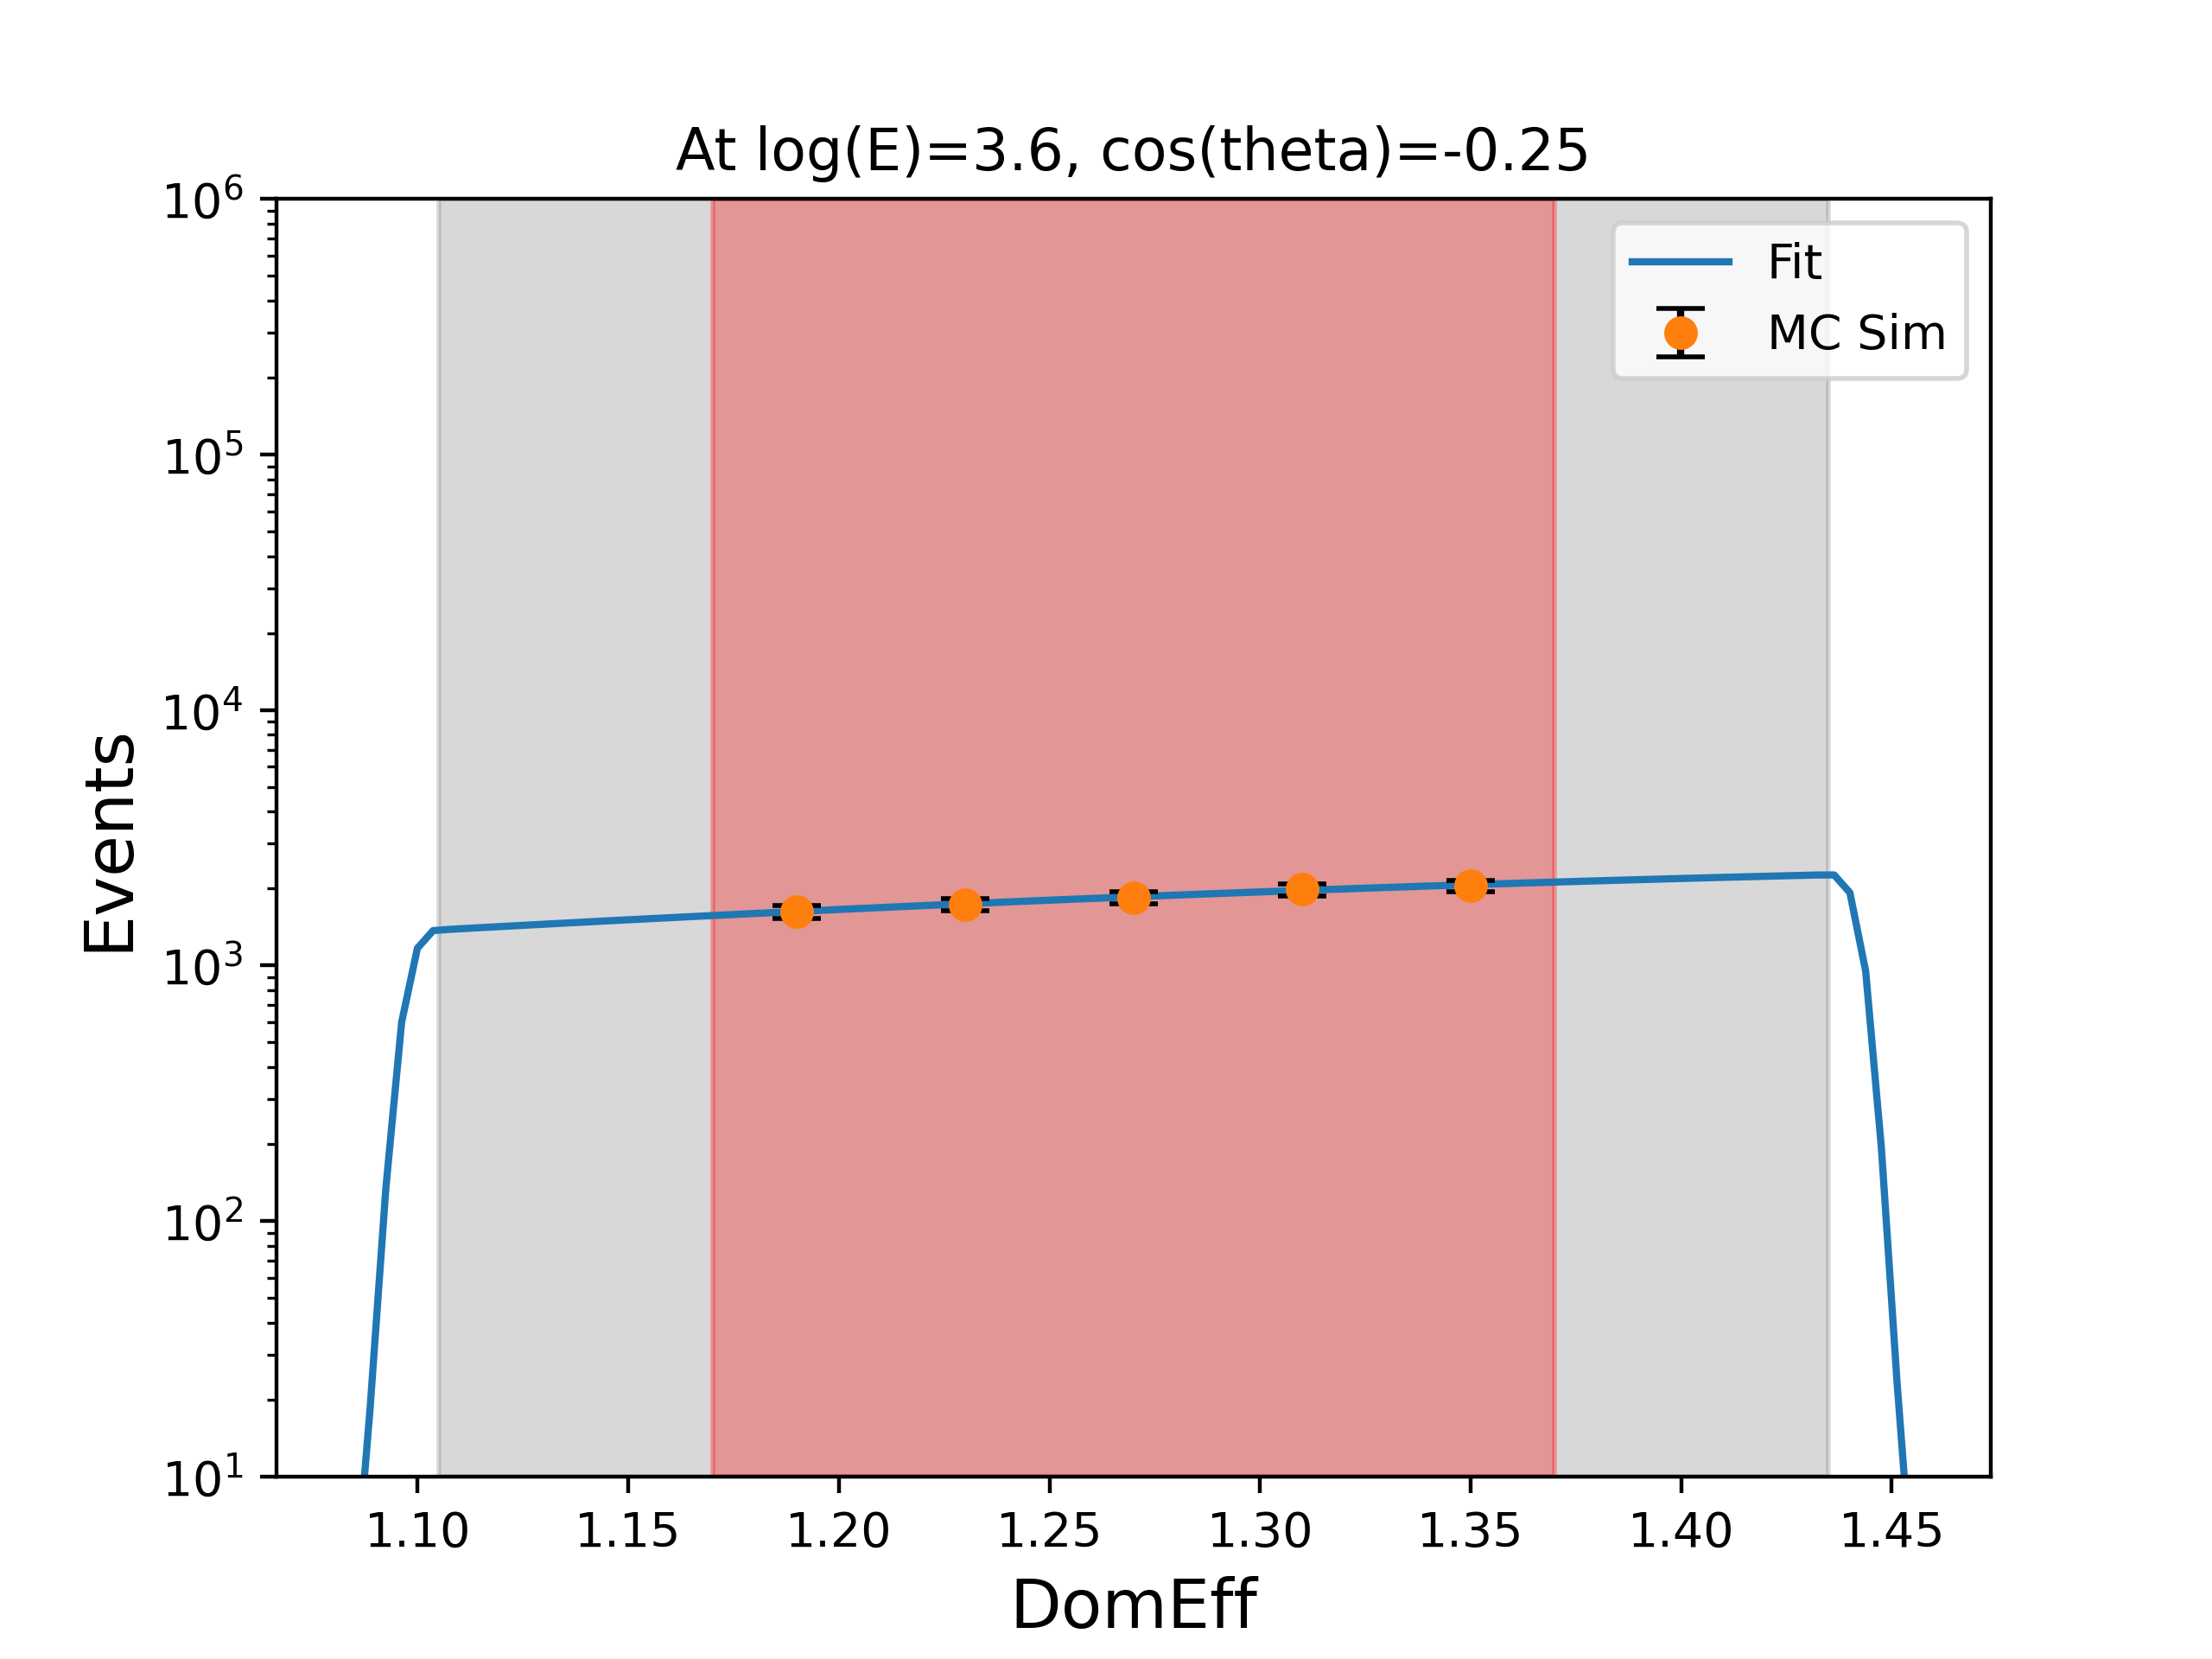
\includegraphics[width=0.8\linewidth]{figures/atmConv_logE_3.6_cosz_-0.25.png}
    \caption{The predicted number of events in reconstructed space for a bin centered at $\log E_{\nu}^{reco}=3.6$ and $\cos\theta_{\nu}^{reco}=0.25$ as a function of the DOM effeciency. The MC data are represented by orange dots, and the spline fit is the trend in blue. The gray shaded region represent the extents of the spline, and the red bands represents prior-allowed region.}\label{fig:domeff_fit}
\end{figure}


\subsection{Bulk Ice}

The bulk ice in the ice is characterised by uncertainties in the absorption and scattering length. 
Initially, every ten meter section of the ice was assigned an absorption length and a scatteing length with some uncertainty. 
Over the 1500 meter span of IceCube, this would require 300 separate nuisance parameters to account for these parameters fully.

This is an overwhelming and intractable quantity. 
For this and similar analyses, a Fourier decomposition of the depth ($x$) dependence of the absorption and scattering is used instead, as described in Ref~\cite{Aartsen_2019_snow}: 
\begin{equation}
    \dfrac{1}{2}\log\left(\text{Abs} \times \text{Sca}\right) = \dfrac{A_{0}}{2} +\sum\limits_{n=1}^{N}A_{n} \sin\left(\dfrac{2\pi nx}{L} + \phi_{n}\right)
\end{equation}
where $A_{n}$ and $\phi_{n}$ are amplitudes and phases for the $n$'th term in the series expansiion, $L$ is the vertical extent of IceCube, and \textit{Abs} and \textit{Sca} are the in-ice absorption and scattering lengths. 


To calibrate these amplitudes and phases and to determine the covariance between them, we use the IceCube in-situ flasher data~\cite{Aartsen_2013}. 
These use the 12 on-board LEDs mounted in the housings of each DOM. 
The LEDs on all DOMs of string 63 are flashed, and then the measured light throughout IceCube, minus string 63, is logged. 
Then, PPC simulations were carried out for various, perturbed, ice models were performed. 
PPC simulations were performed by perturbing the amplitudes and phases for the first four modes in the Fourier series expansion of the depth dependence of absorption and scattering in the bulk ice.
PPC simulations were also performed by perturbing various combinations of these modes. 
These PPC simulations were used, in conjunction with the measured flasher data, to quantify the likelihood of the observed data assuming different ice models,

For each amplitude and phase, these likelihoods were calculated for icemodels where the amplitudes of the first five fourier modes and the first fourier phases were shifted. 
These values were shited large amounts first, from which an approximate minimum was determined. 
Then, more granular PPC simulations were carried out by varrying these amplitudes and phases about the approximate centers. 

For each amplitude and phase a quadratic fit was then done to the log likelihood distributions, 
\begin{equation}
    \mathcal{L}(\eta_{i}) = A_{i}\eta_{i}^{2} + B_{i}\eta_{i} + C_{i}
\end{equation}
where $\eta_{i}$ is for any one amplitude or phase. These fits are shown in Figure FIG. 
A similar scan was then done for combinations of nuisance parameters by shifting each possible pairing of them by amounts proportional to the widths of the nuisance parameters. 

For a correlated set of nuisance parameters $\vec{\eta}$, the prior penalty of the likelihood function is equal to 
\begin{equation}
    \mathcal{L} = \vec{\eta}^{T} \Sigma^{-1} \vec{\eta} + C
\end{equation} 
where $C$ is a constant prefactor to normalize the distribution and $\Sigma$ is the covariance.
The inverse of the covariance matrix, $\Sigma^{-1}$, is also known as the Hessian matrix, and so to fit to the covariance it is easiest to fit first to the Hessian. 
In order for the prior penalty function to normalizable, both the covariance matrix and the hessian must be real-valued and positive semi-definite: all eigenvalues and its determinant must be greater than or equal to zero. 
A consequence of this is that the Hessian can be written as 
\begin{equation}
    \Sigma^{-1} = H = LL^{T},
\end{equation} 
where $L$ is a lower-diagonal matrix. 
We can therefore parametrize any Hessian matrix $H$ using values occupying the lower-diagonal of such a matrix $L$. This takes $n(n-1)/2$ values, where $n$ is the rank of the covariance. 

For a given lower-diagonal matrix $\bvec{L}$, we minimize the cauchy robust loss function given by 
\begin{equation}
    M(\bvec{L}) = \sum_{i}^{m}\log\left[ 1 +  \left(\mathcal{L}_{i} - (\vec{\eta}_{i})^{T} \bvec{L}\bvec{L}^{T} \vec{\eta}_ {i} \right)^{2}\right]
\end{equation}
for the $m$ sampled ice models where $\vec{\eta}_{i}$ is the $i$'th sampled set of nuisance parameters at which a log likelihood of $\mathcal{L}_{i}$ was recovered through PPC simulation. 
This likelihood function, which has been used in previous IceCube analyses~\cite{icecube_lowe}, was chosen such that bad fits far off the true likelihood contours do not negatively effect the fit.  
The fit, despite running over forty-five parameters, was found to be extremely stable and fast. The fit Hessian $H=\bvec{L}\bvec{L}^{T}$ is show in Figure~\ref{fig:hessian} (left) and the corrlation matrix (right).
\begin{figure}
    \centering
    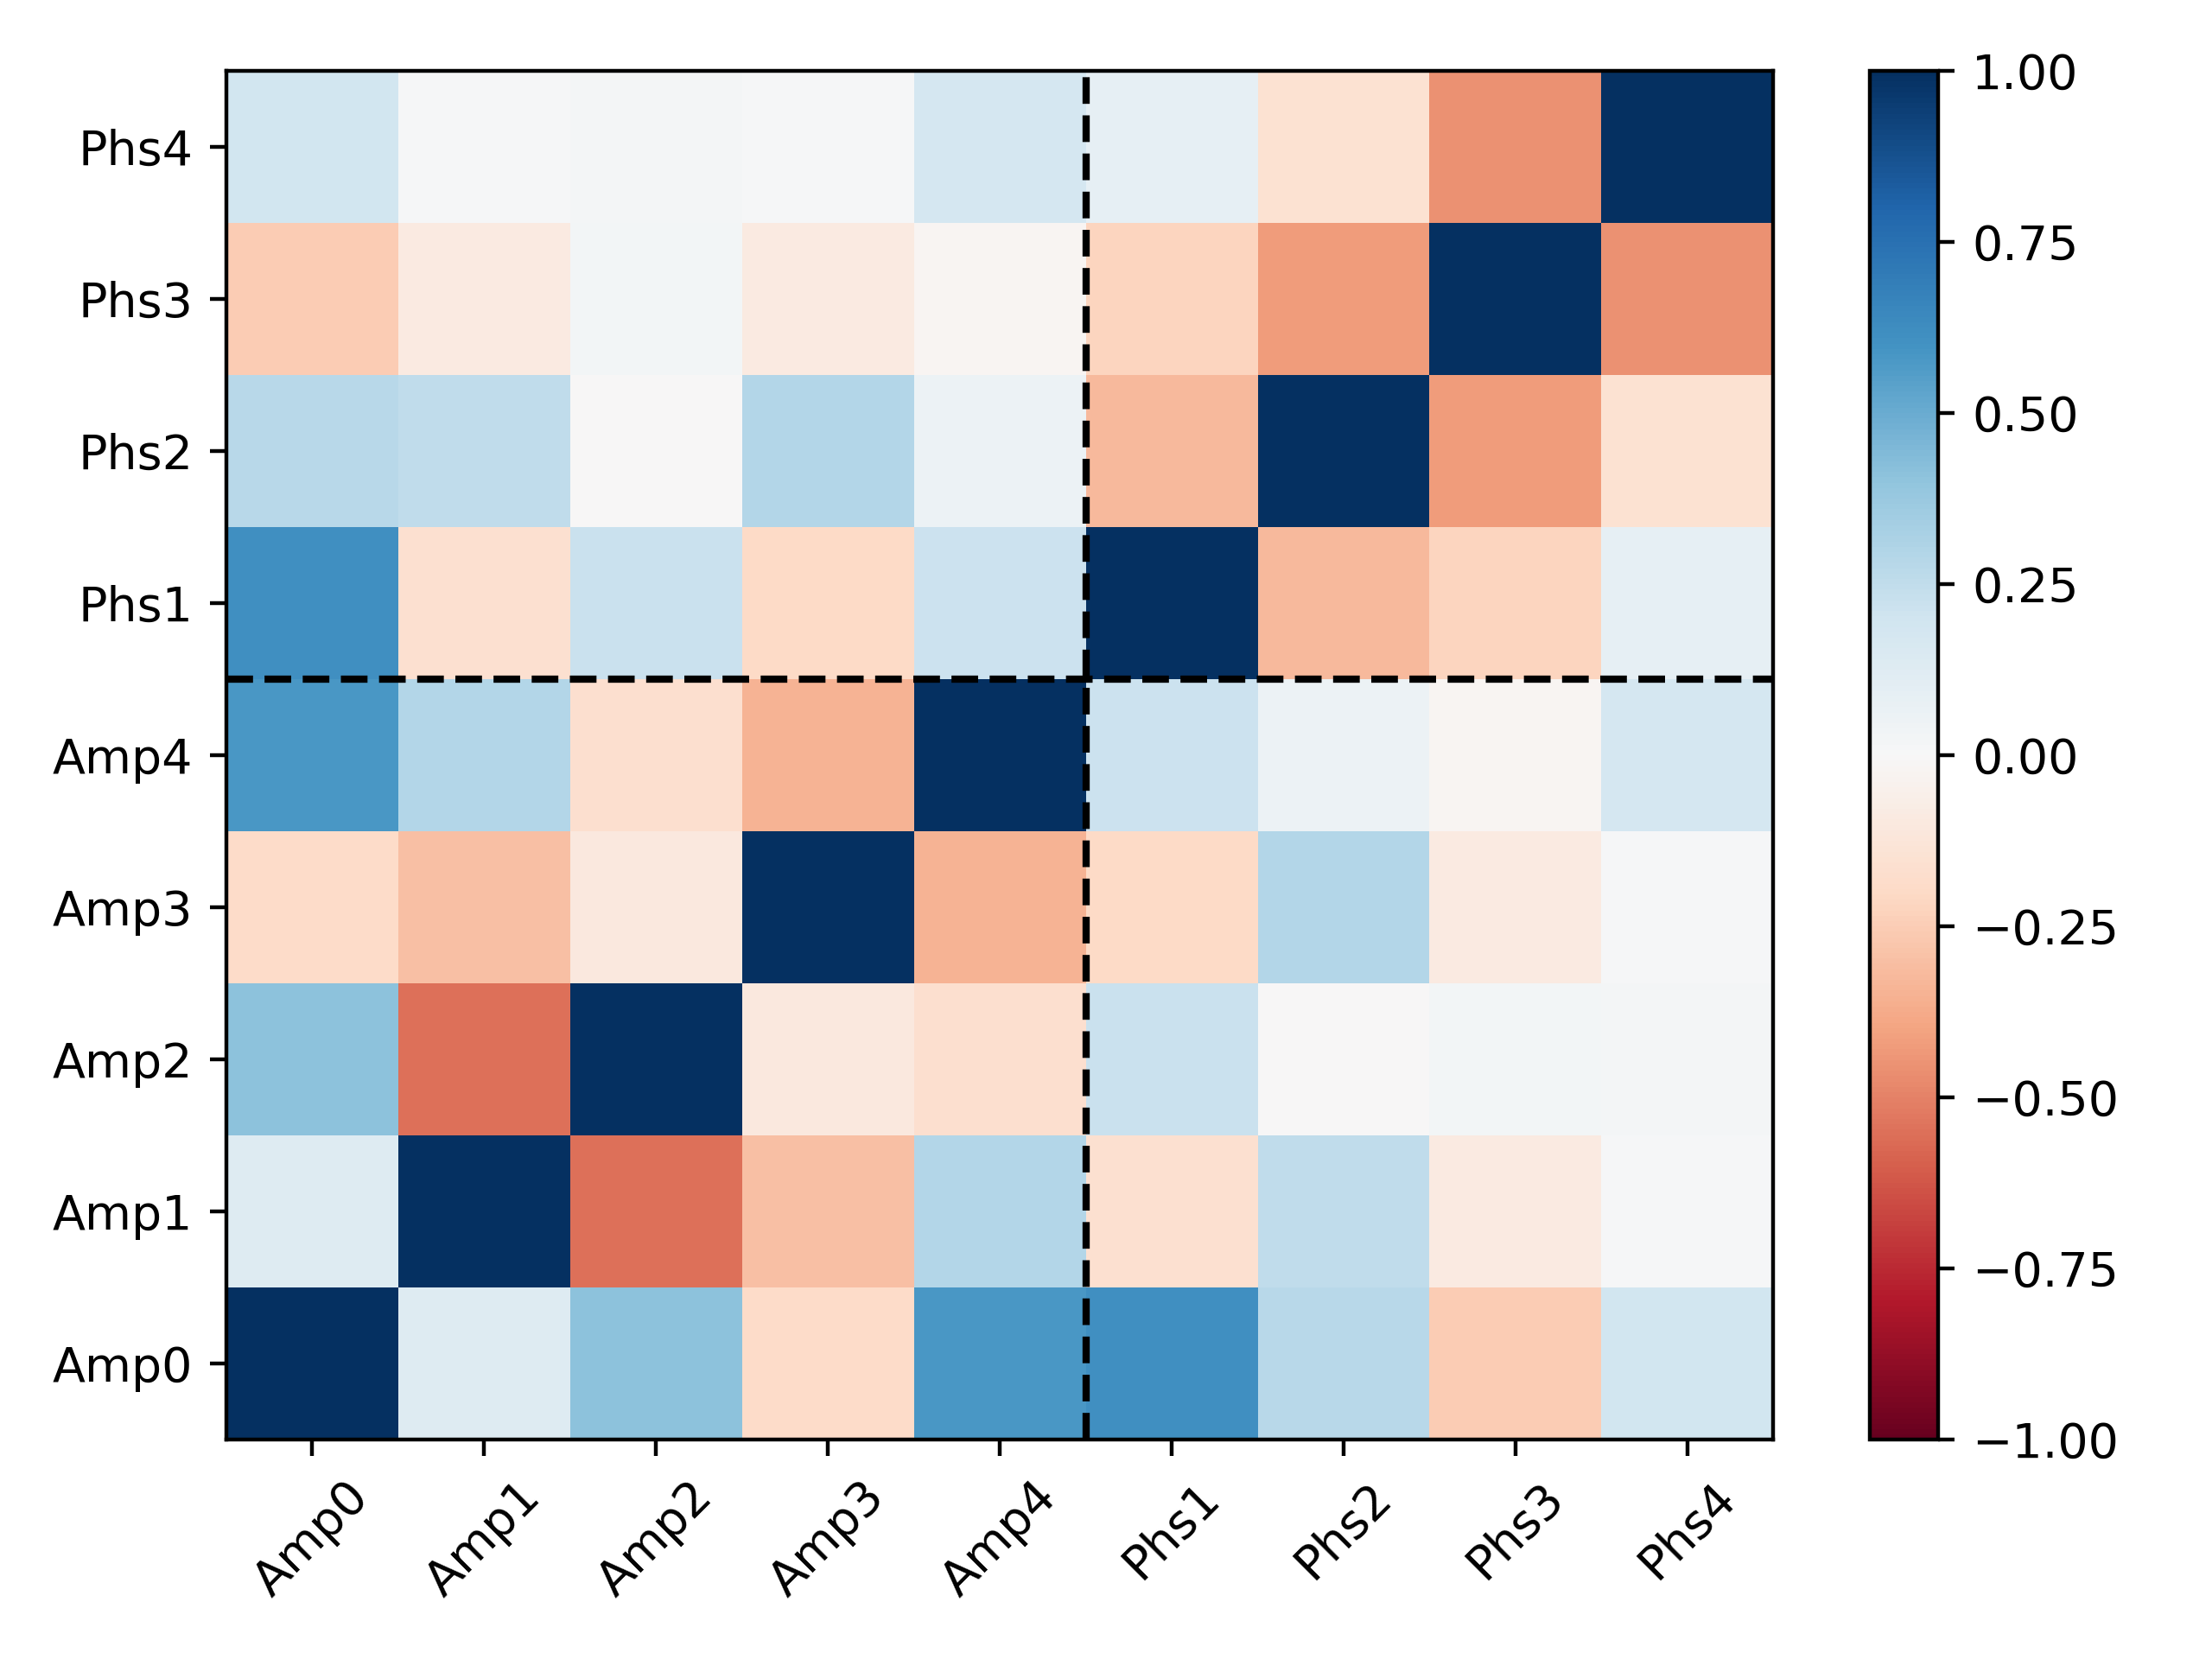
\includegraphics[width=0.45\linewidth]{figures/hessian.png}%
    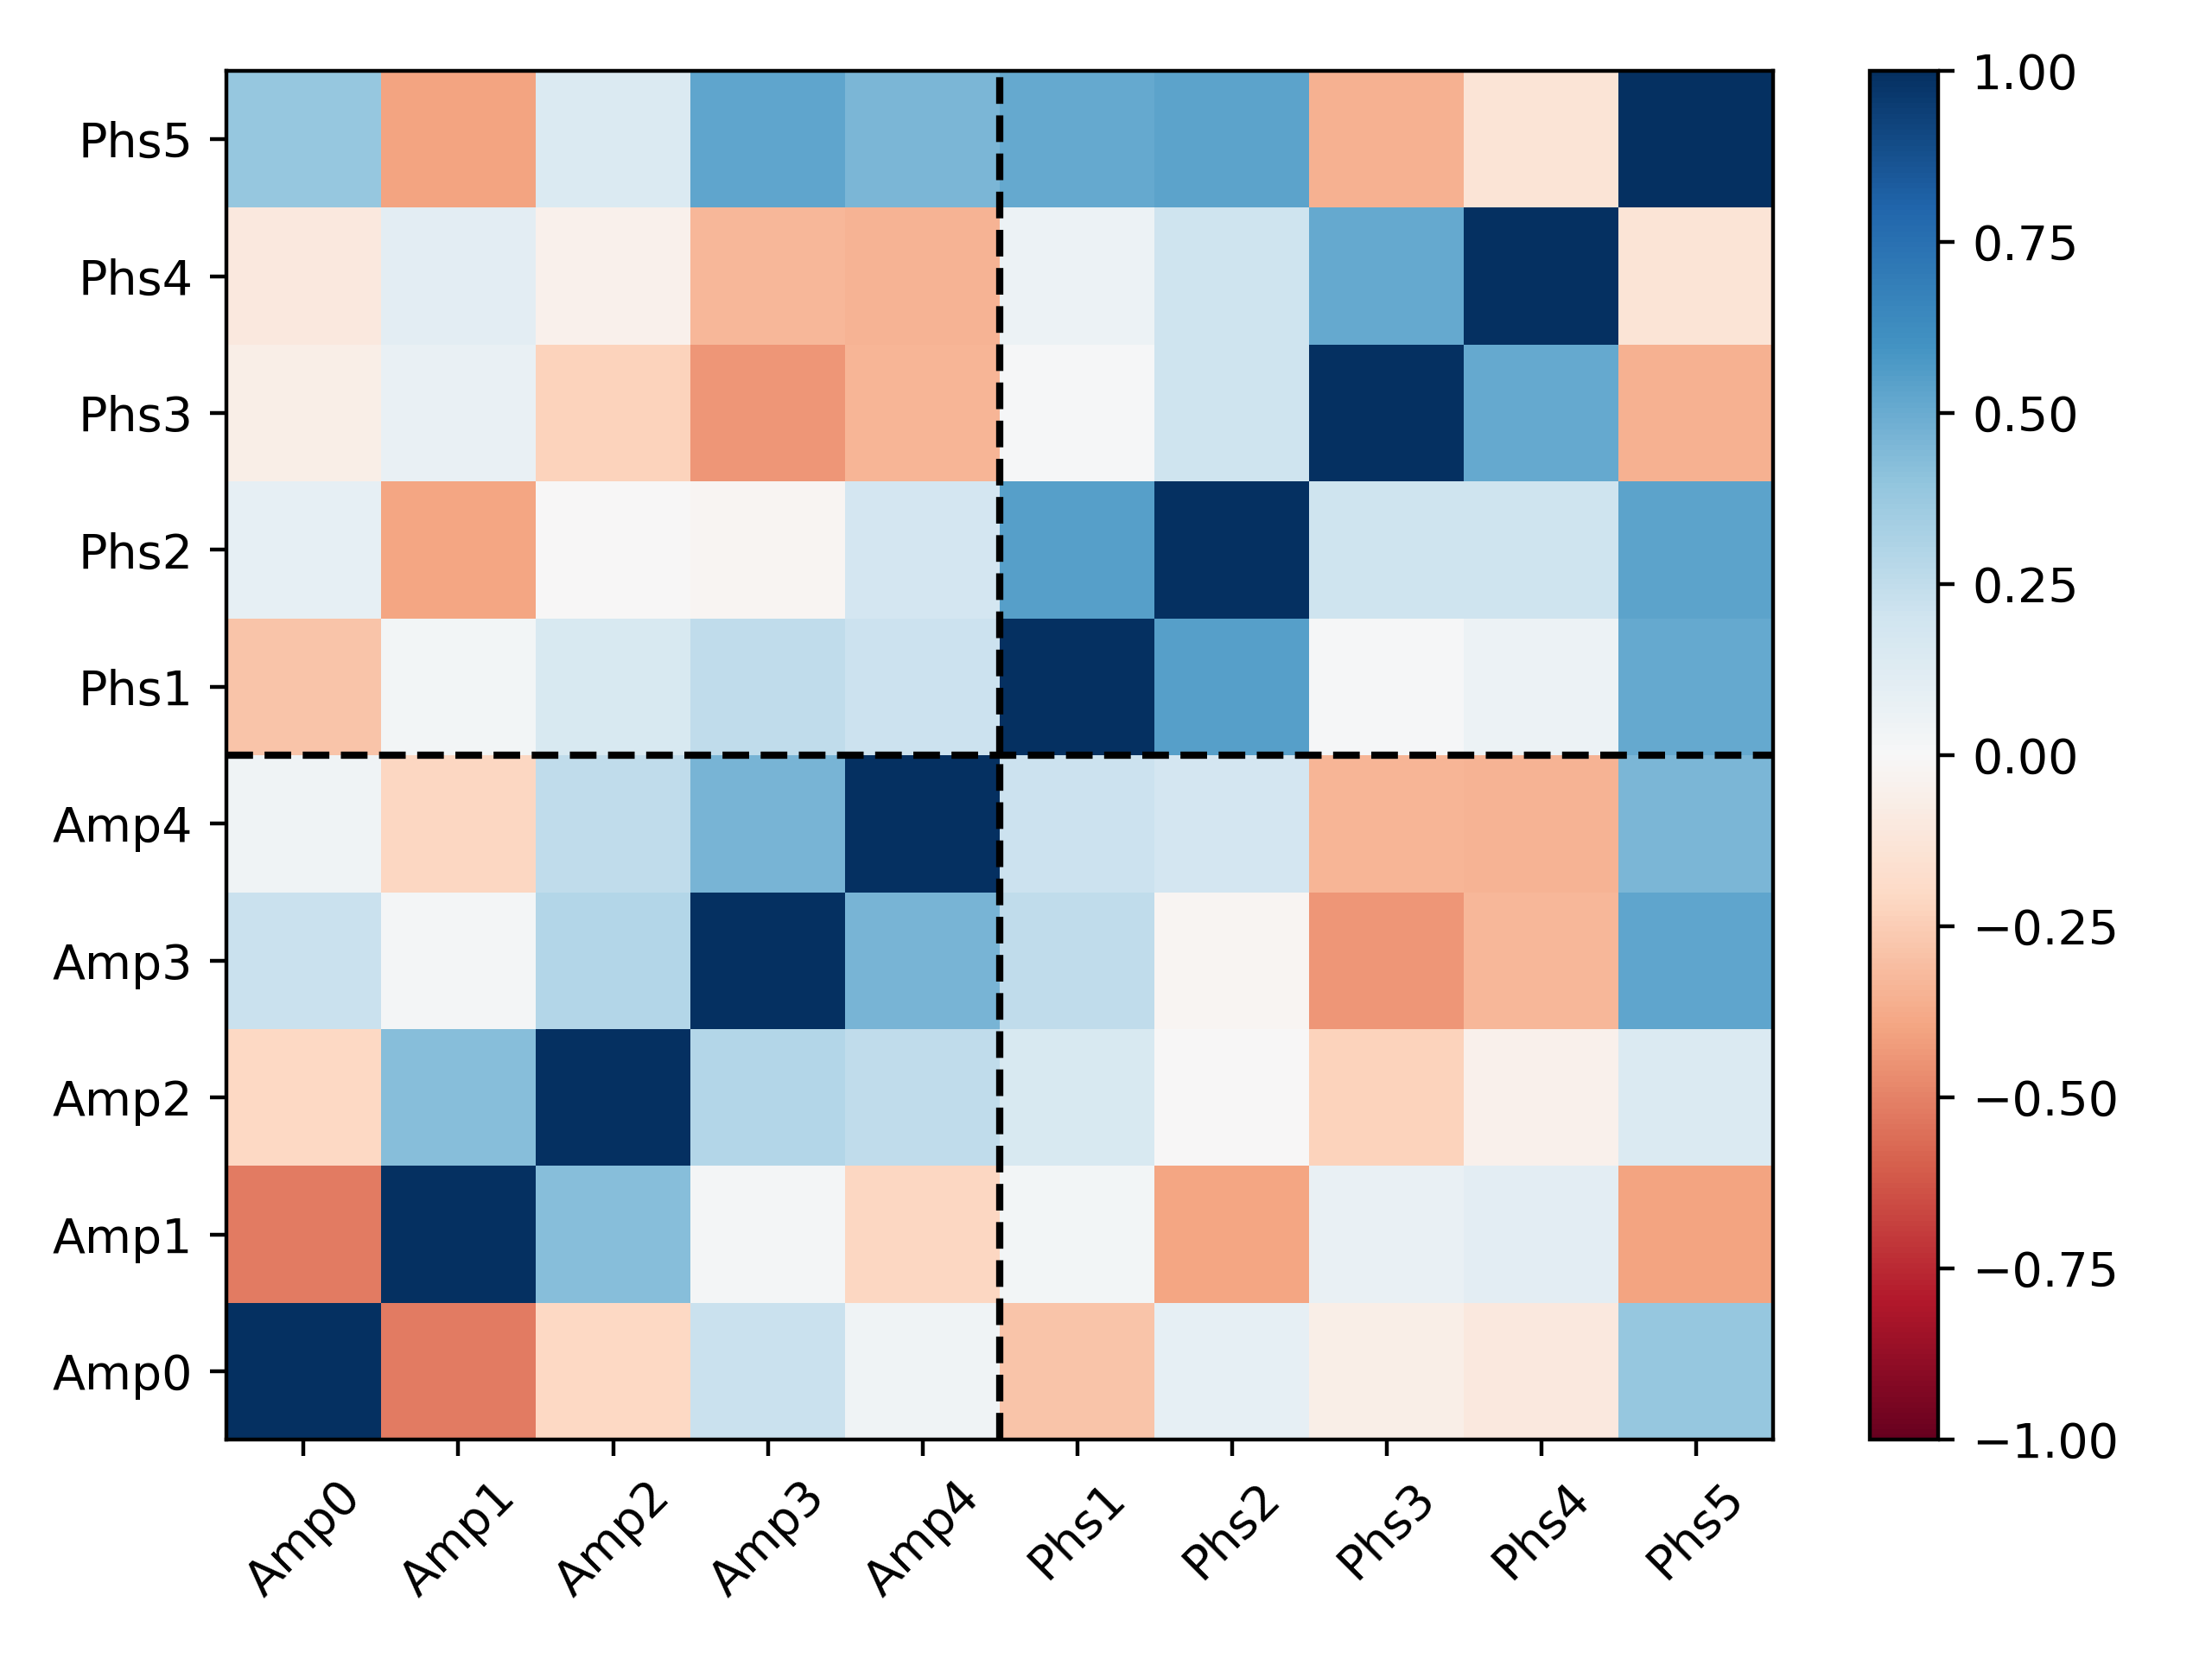
\includegraphics[width=0.45\linewidth]{figures/covariance.png}
    \caption{The fit hessian matrix (left), in nuisance parameter space, for the first five amplitudes and first four phases, and the correlation matrix(right) determined by inverting the hessian.}\label{fig:hessian}
\end{figure}

Using these the expected varriation of ice models can be calculated. 
Five thousand random ice models were drawn, using the correlation matrix and the fit widths of the amplitudes and phases, and are shown in Figure~\ref{fig:envelope}.

\begin{figure}
    \centering
    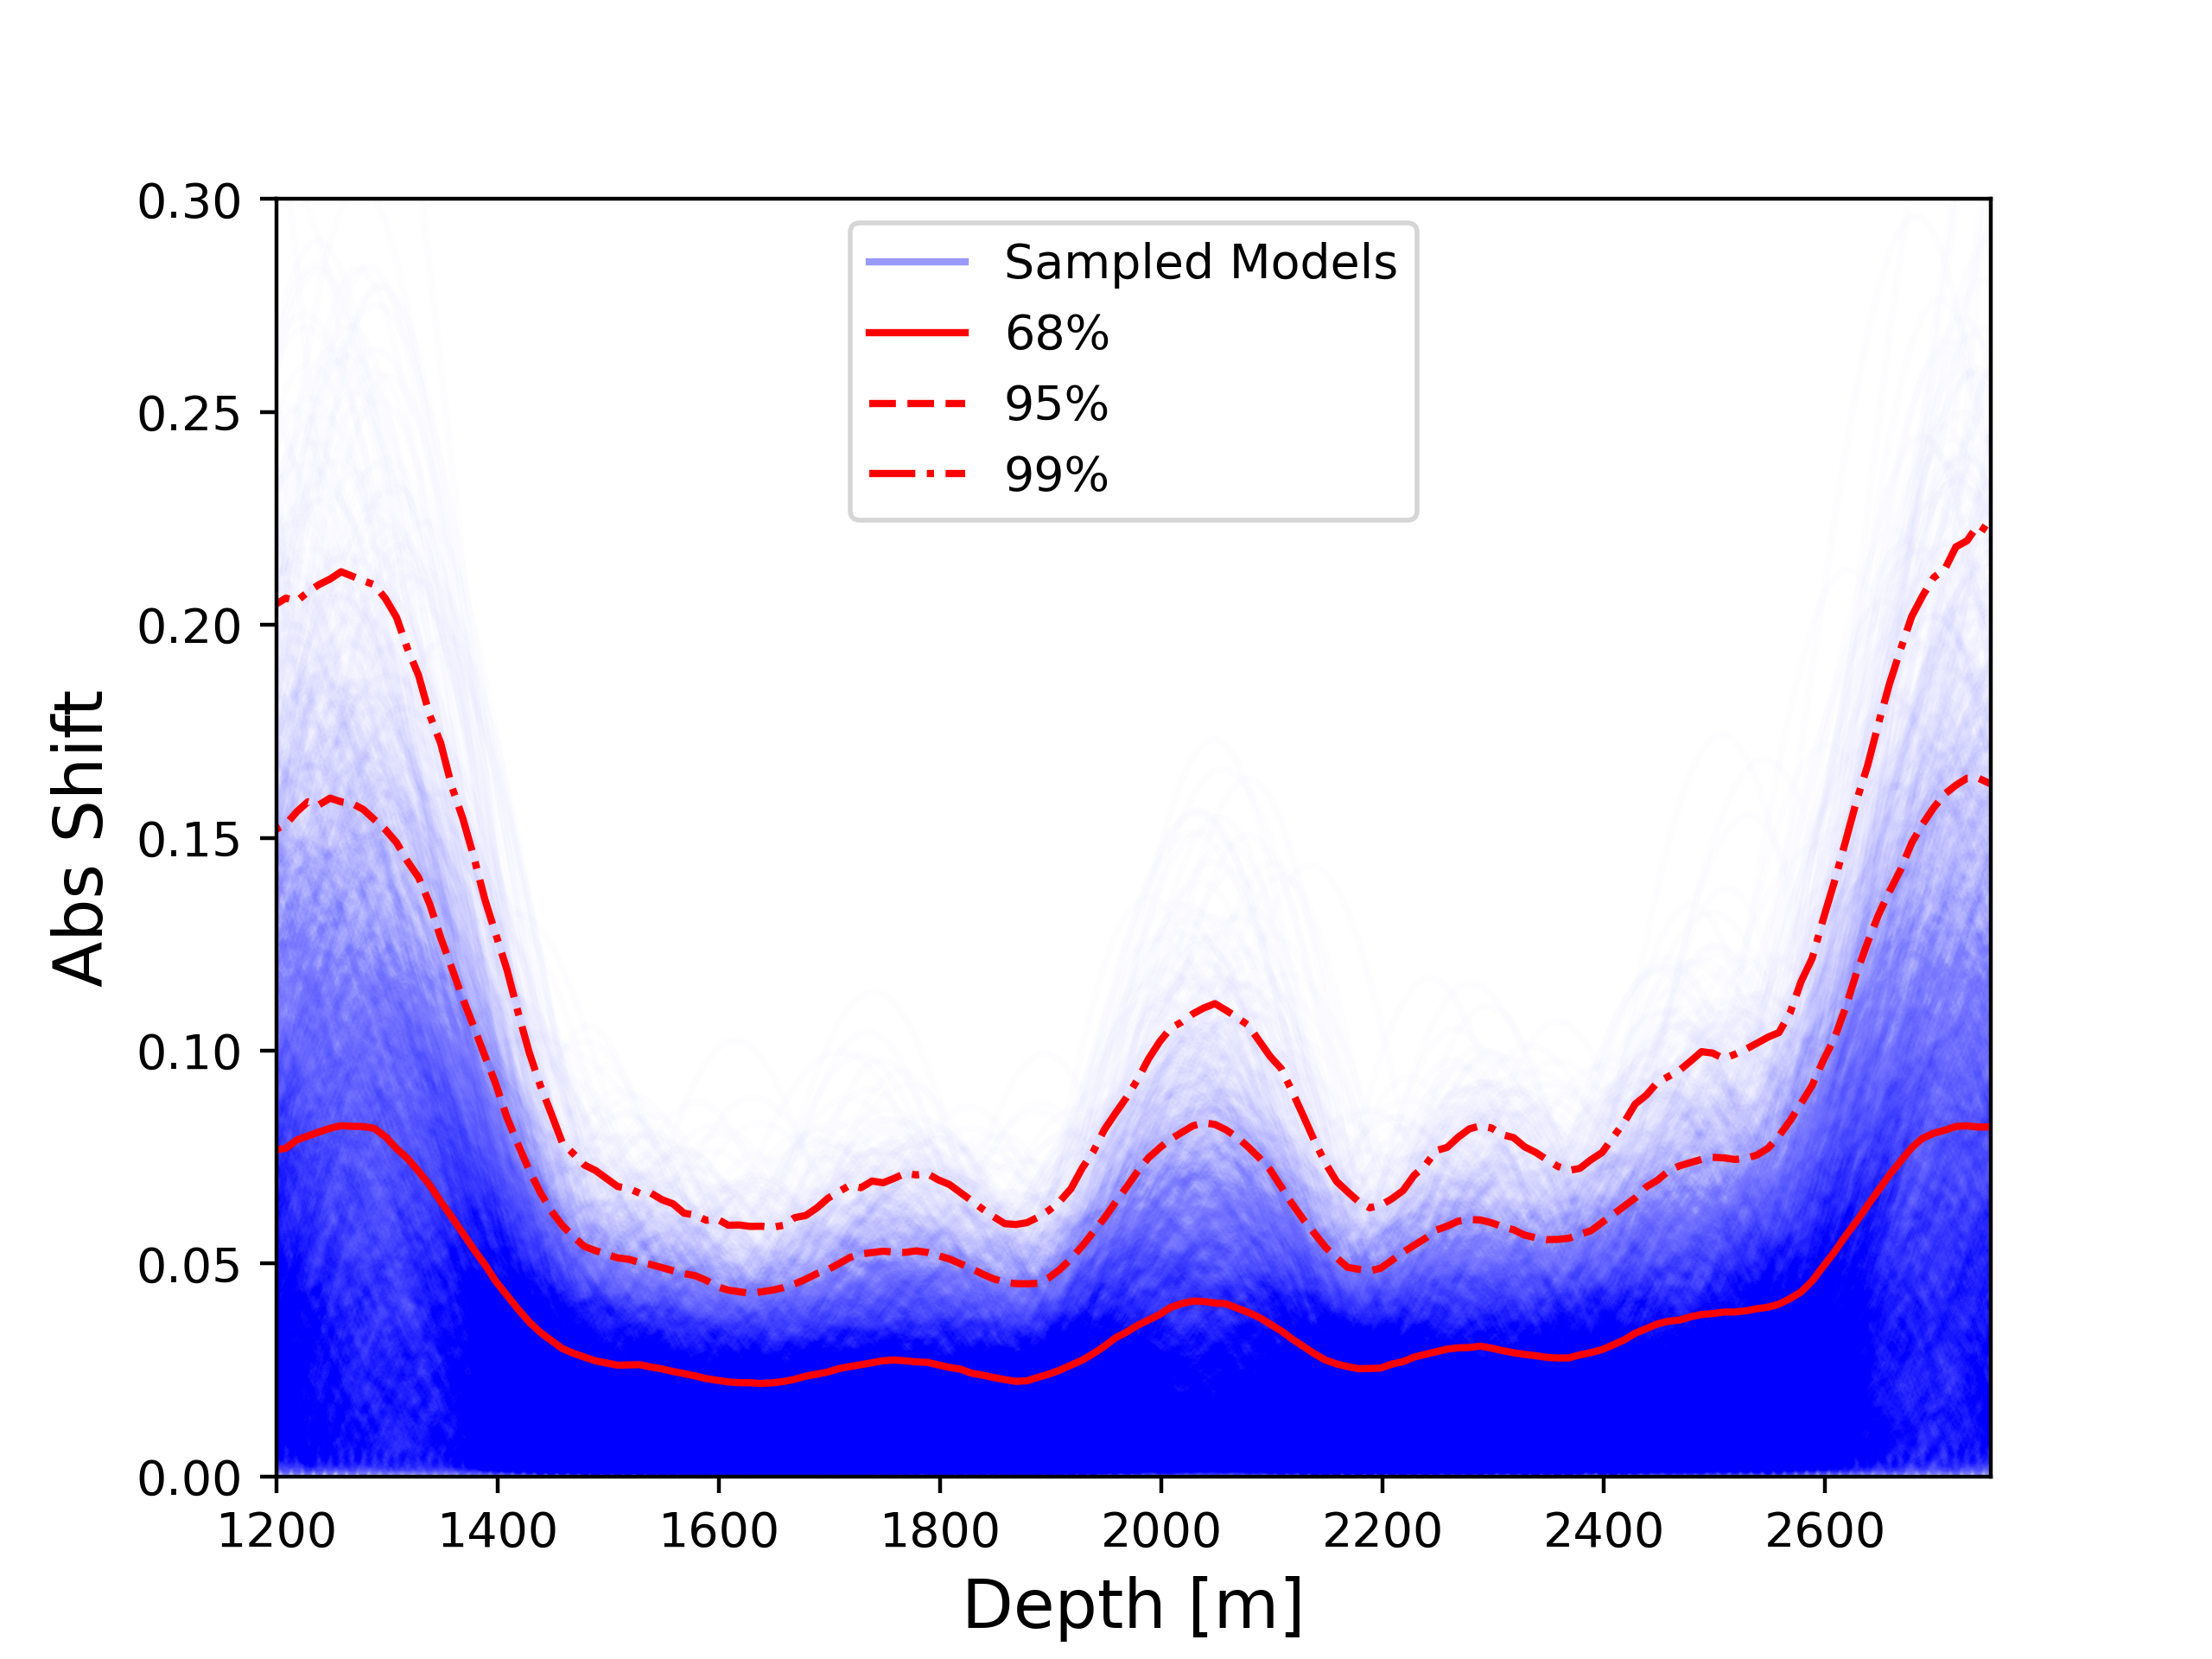
\includegraphics[width=0.8\linewidth]{figures/icemodel_smooth.png}
    \caption{The results of sampling five thousand ice models using the fit correlation matrix and widths for the amplitudes and phases. A solid red line is drawn, below which the fractional shift of the absorption length of 68\% of sampled models lie. Similar lines for 95\% and 99\%. IceCube lies between 1500 and 2500 meters of depth. The bump in the middle lines up with the dust layer in IceCube, and rises at the end are caused by poor constraint due to the physical extent of the detector.}\label{fig:envelope}
\end{figure}

The widths on the icemodels were then used in an application of the SnowStorm technique. 
A purpose-build Monte Carlo sample was prepared generating only events that would yield cascades; since we were not interested in developing a sample to test event selection efficiency, background events were not included. 
This sample was generated using the same procedure as described in Chapter~\ref{chapter:gen}. 
Energies were all sampled at according to a power law with a spectral index $\gamma=-2$.
Sub-samples were prepared spanning different energy regimes and using different numbers of events per file, injection cylinder sizes, and events per model. 
The full ensemble of event generation parameters are shown in Table~\ref{table:mc}.

\begin{table}
    \centering
    \rowcolors{2}{gray!25}{white}
    \begin{tabular}{c | ccc ccc ccc c}\rowcolor{blue!25}
            & 1001 & 1002 & 1003 & 1004 & 1005 & 1006 & 1007 & 1008 & 1009 & 1010 \\\hline
        
    Flavor  &$\nu_{e}$ &$\nu_{\mu}$ &$\nu_{\tau}$ &$\nu_{e}$ &$\nu_{\tau}$ &$\nu_{e}$ &$\nu_{\mu}$ &$\nu_{\tau}$ &$\nu_{e}$ &$\nu_{\tau}$  \\
    Current & NC & NC & NC & CC & CC & NC & NC & NC & CC & CC \\
    Events Per File & \multicolumn{5}{c}{50,000} & \multicolumn{5}{c}{10,000} \\
    $E_{min}$ [GeV] & \multicolumn{5}{c}{100} & \multicolumn{5}{c}{$5e3$} \\
    $E_{max}$ [GeV] & \multicolumn{5}{c}{$5e3$} & \multicolumn{5}{c}{$10e6$}\\
    Zenith Range & \multicolumn{10}{c}{Full Sky}\\
    Cylinder Height & \multicolumn{10}{c}{1400 m}\\
    Cylinder Radius & \multicolumn{5}{c}{700 m} & \multicolumn{5}{c}{750 m} \\
    Sampled $\gamma$ & \multicolumn{10}{c}{-2} \\
    Events Per Model & \multicolumn{5}{c}{5} & \multicolumn{5}{c}{10} 
    \end{tabular}
    \caption{MC generation scecifications for the snowstorm cascades sample}\label{table:mc}
\end{table}

From these, splits were applied to the full sample and 2D linear gradients were calculated. 
Photospline~\cite{WHITEHORN20132214} was then used to perform spline fits of the 2D gradients to smooth out MC statistical varriance. 
A table of spline fits is shown below in Figure\ref{fig:gradients}. 

\begin{figure}
    \centering
    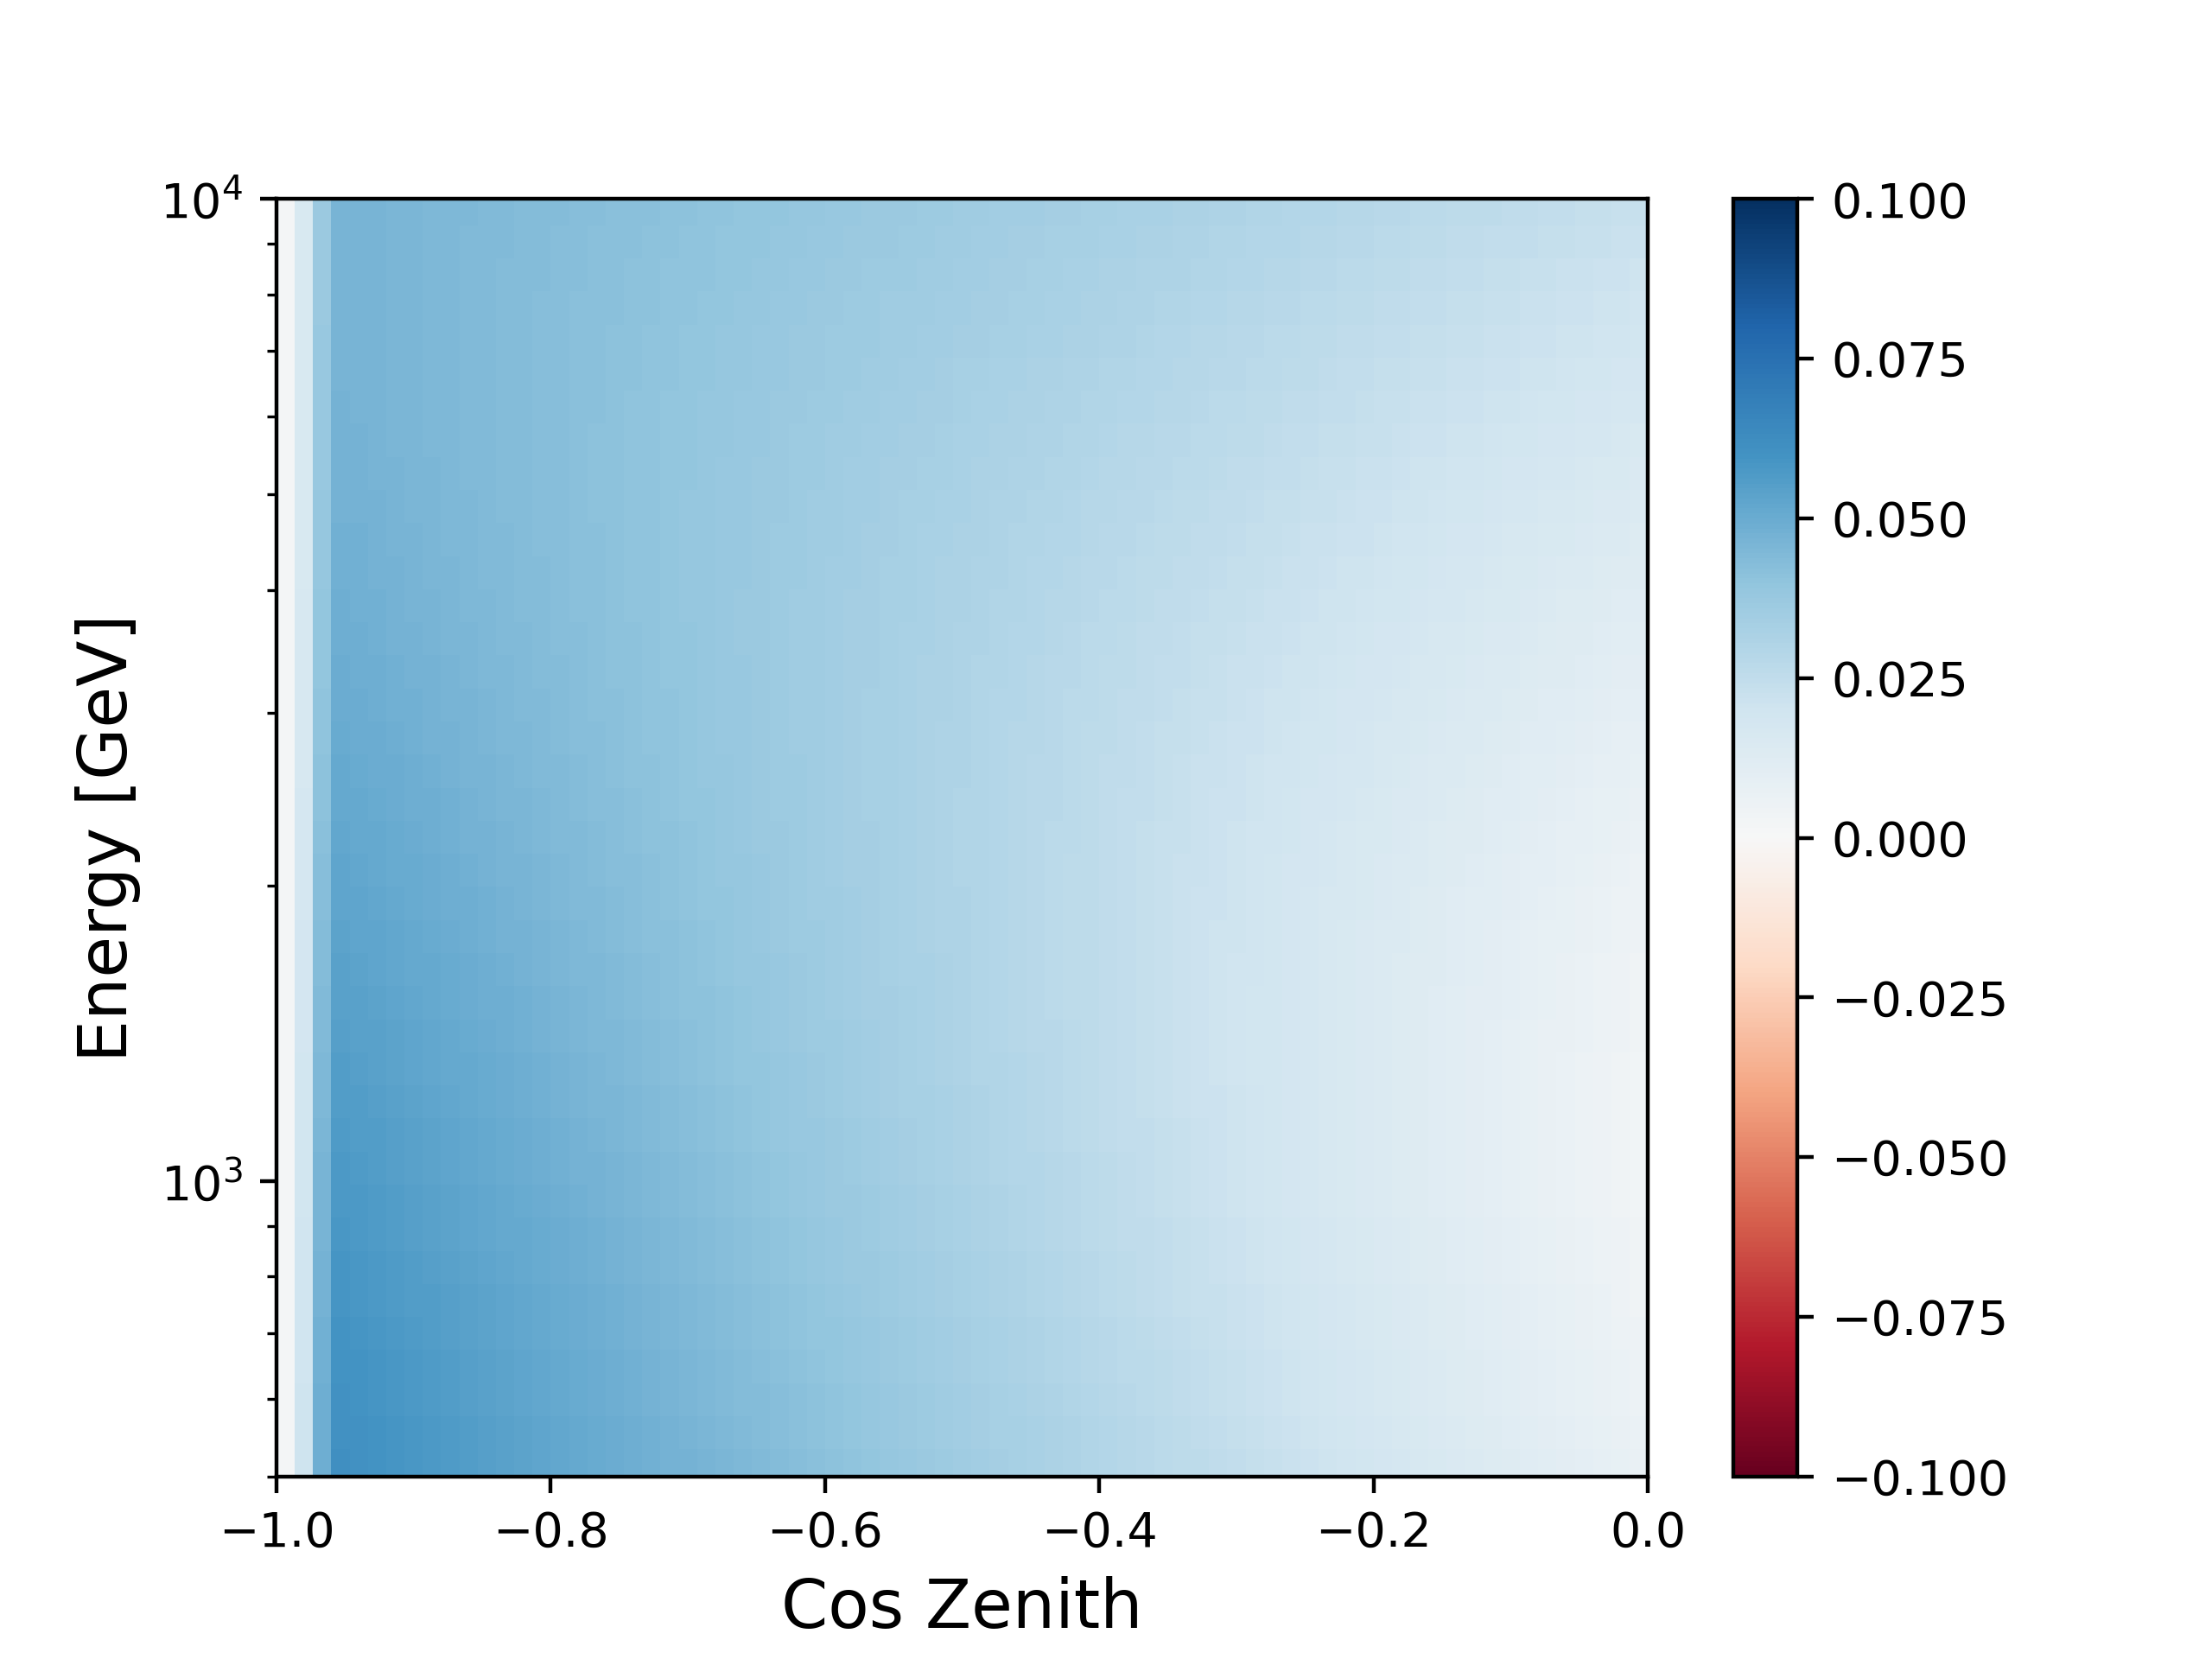
\includegraphics[width=0.3\linewidth]{figures/spline_amp00_gradient.png}%
    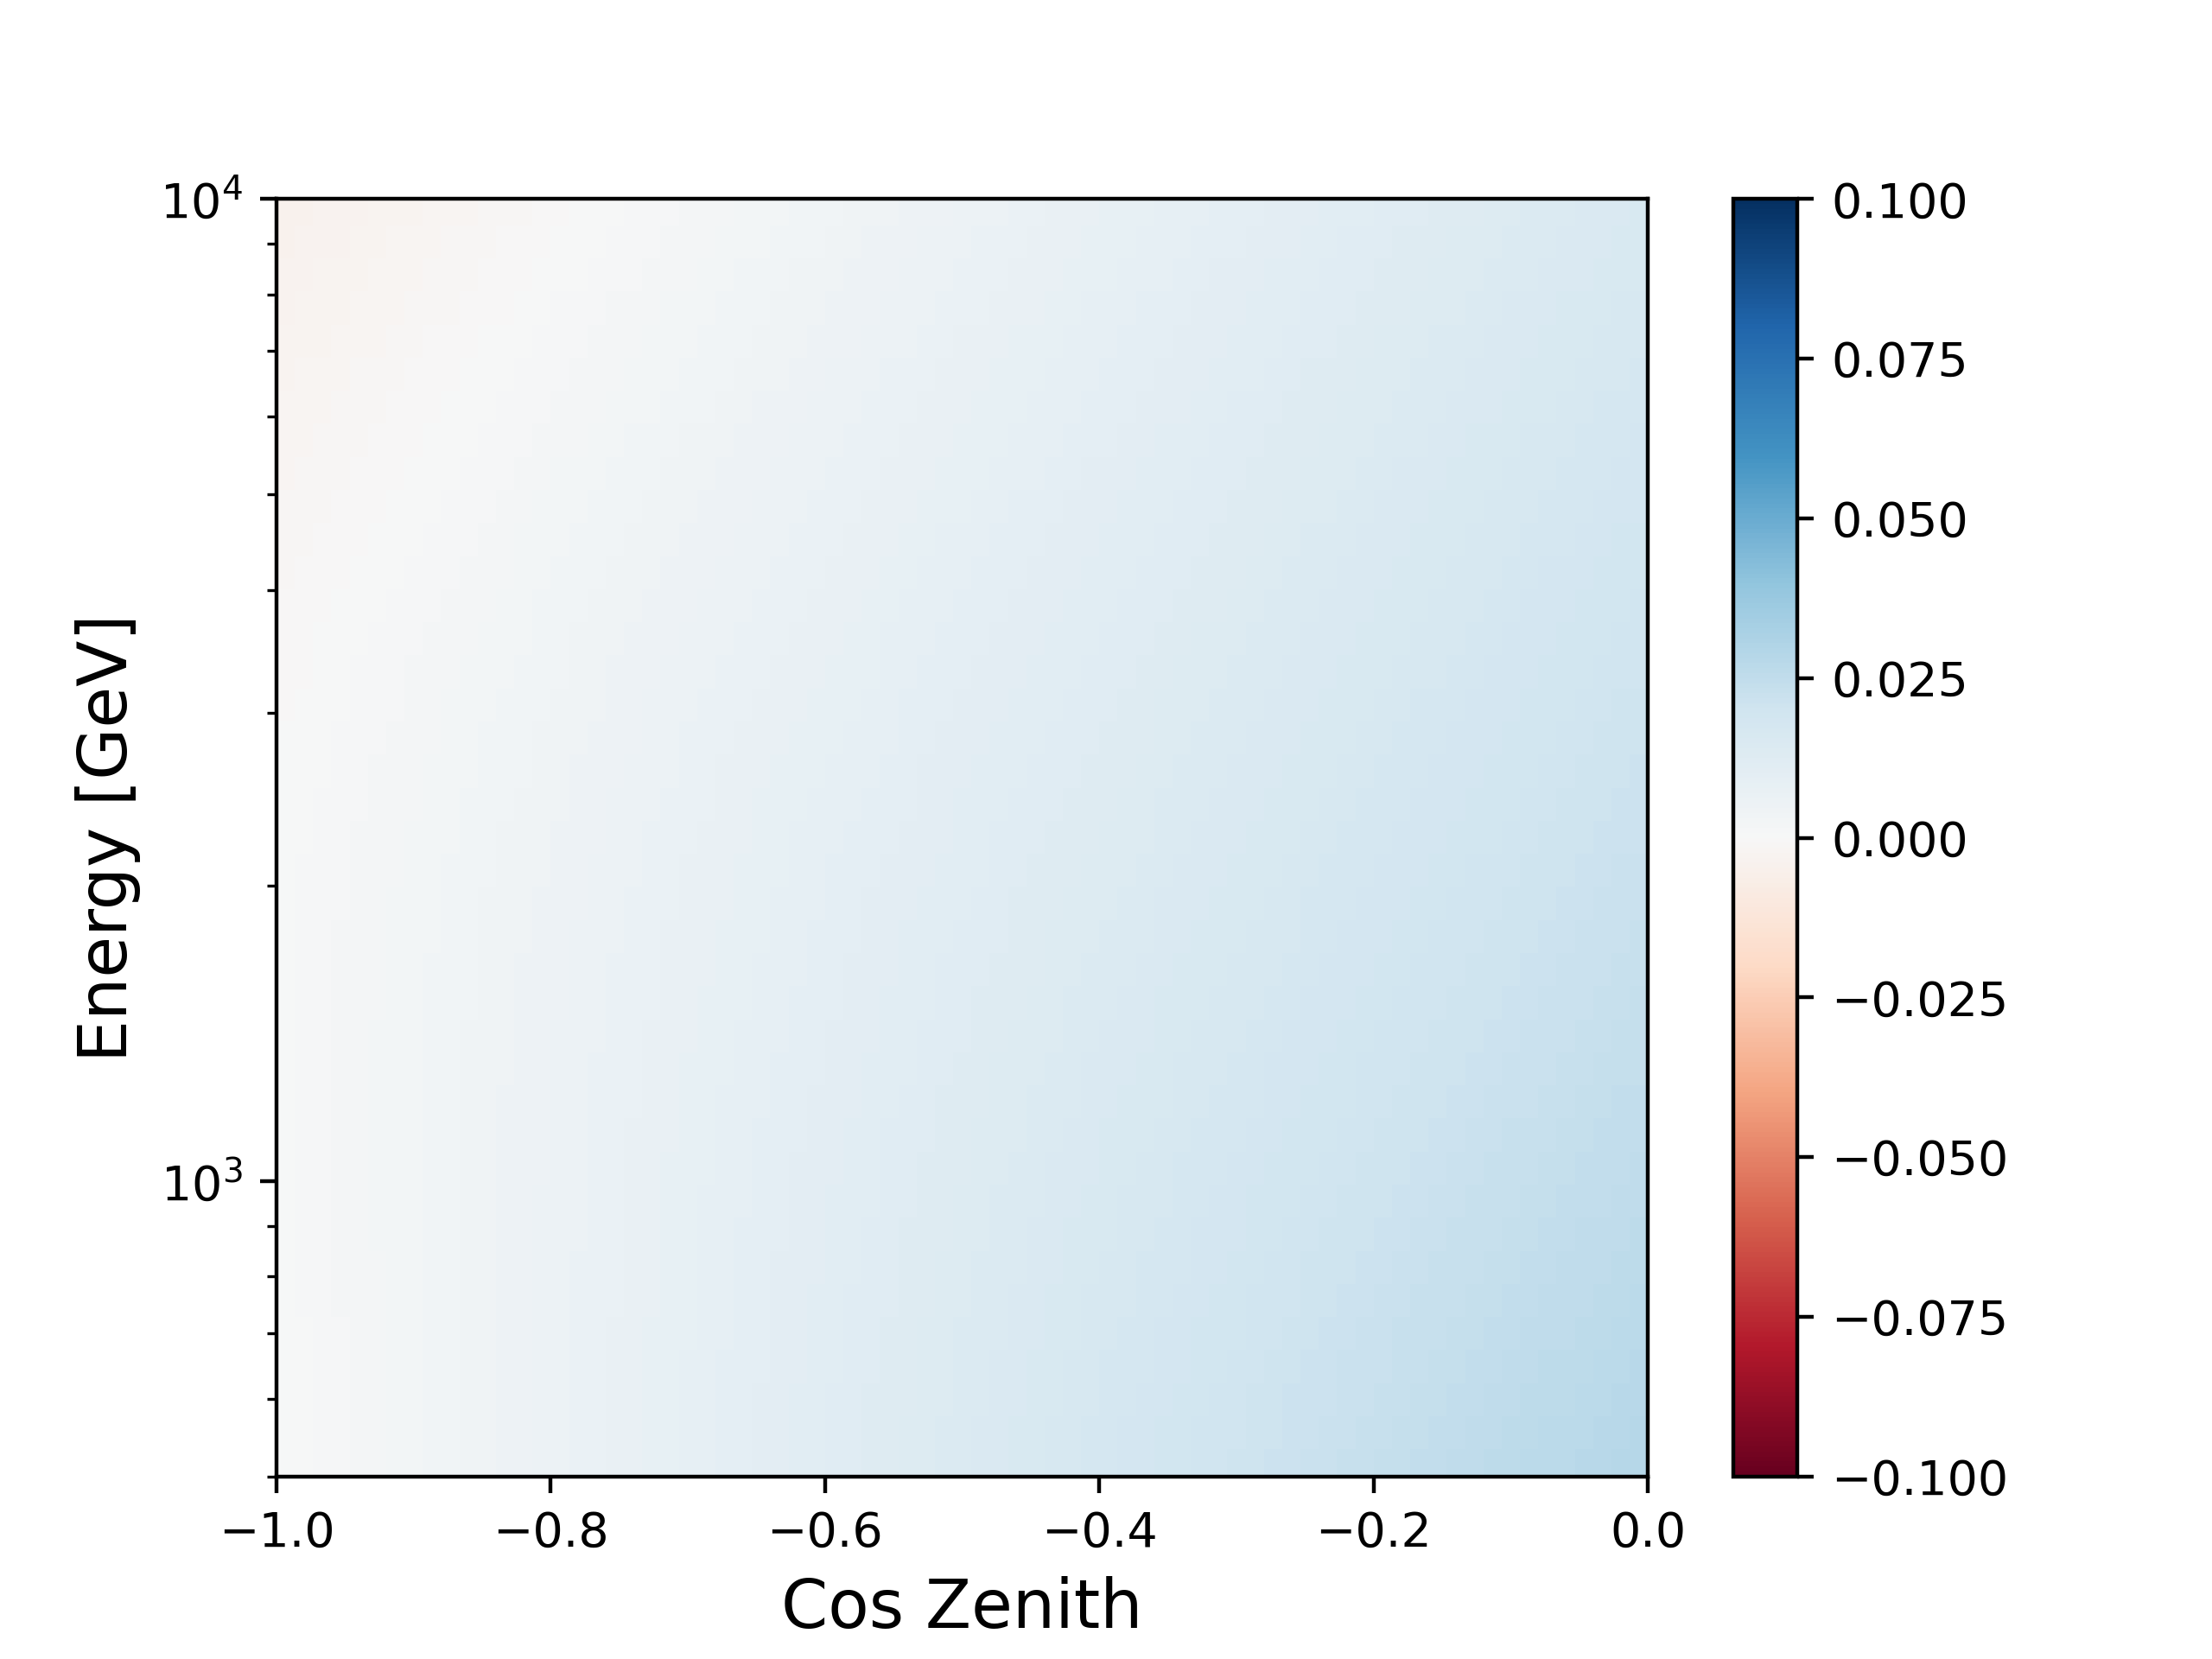
\includegraphics[width=0.3\linewidth]{figures/spline_amp01_gradient.png}%
    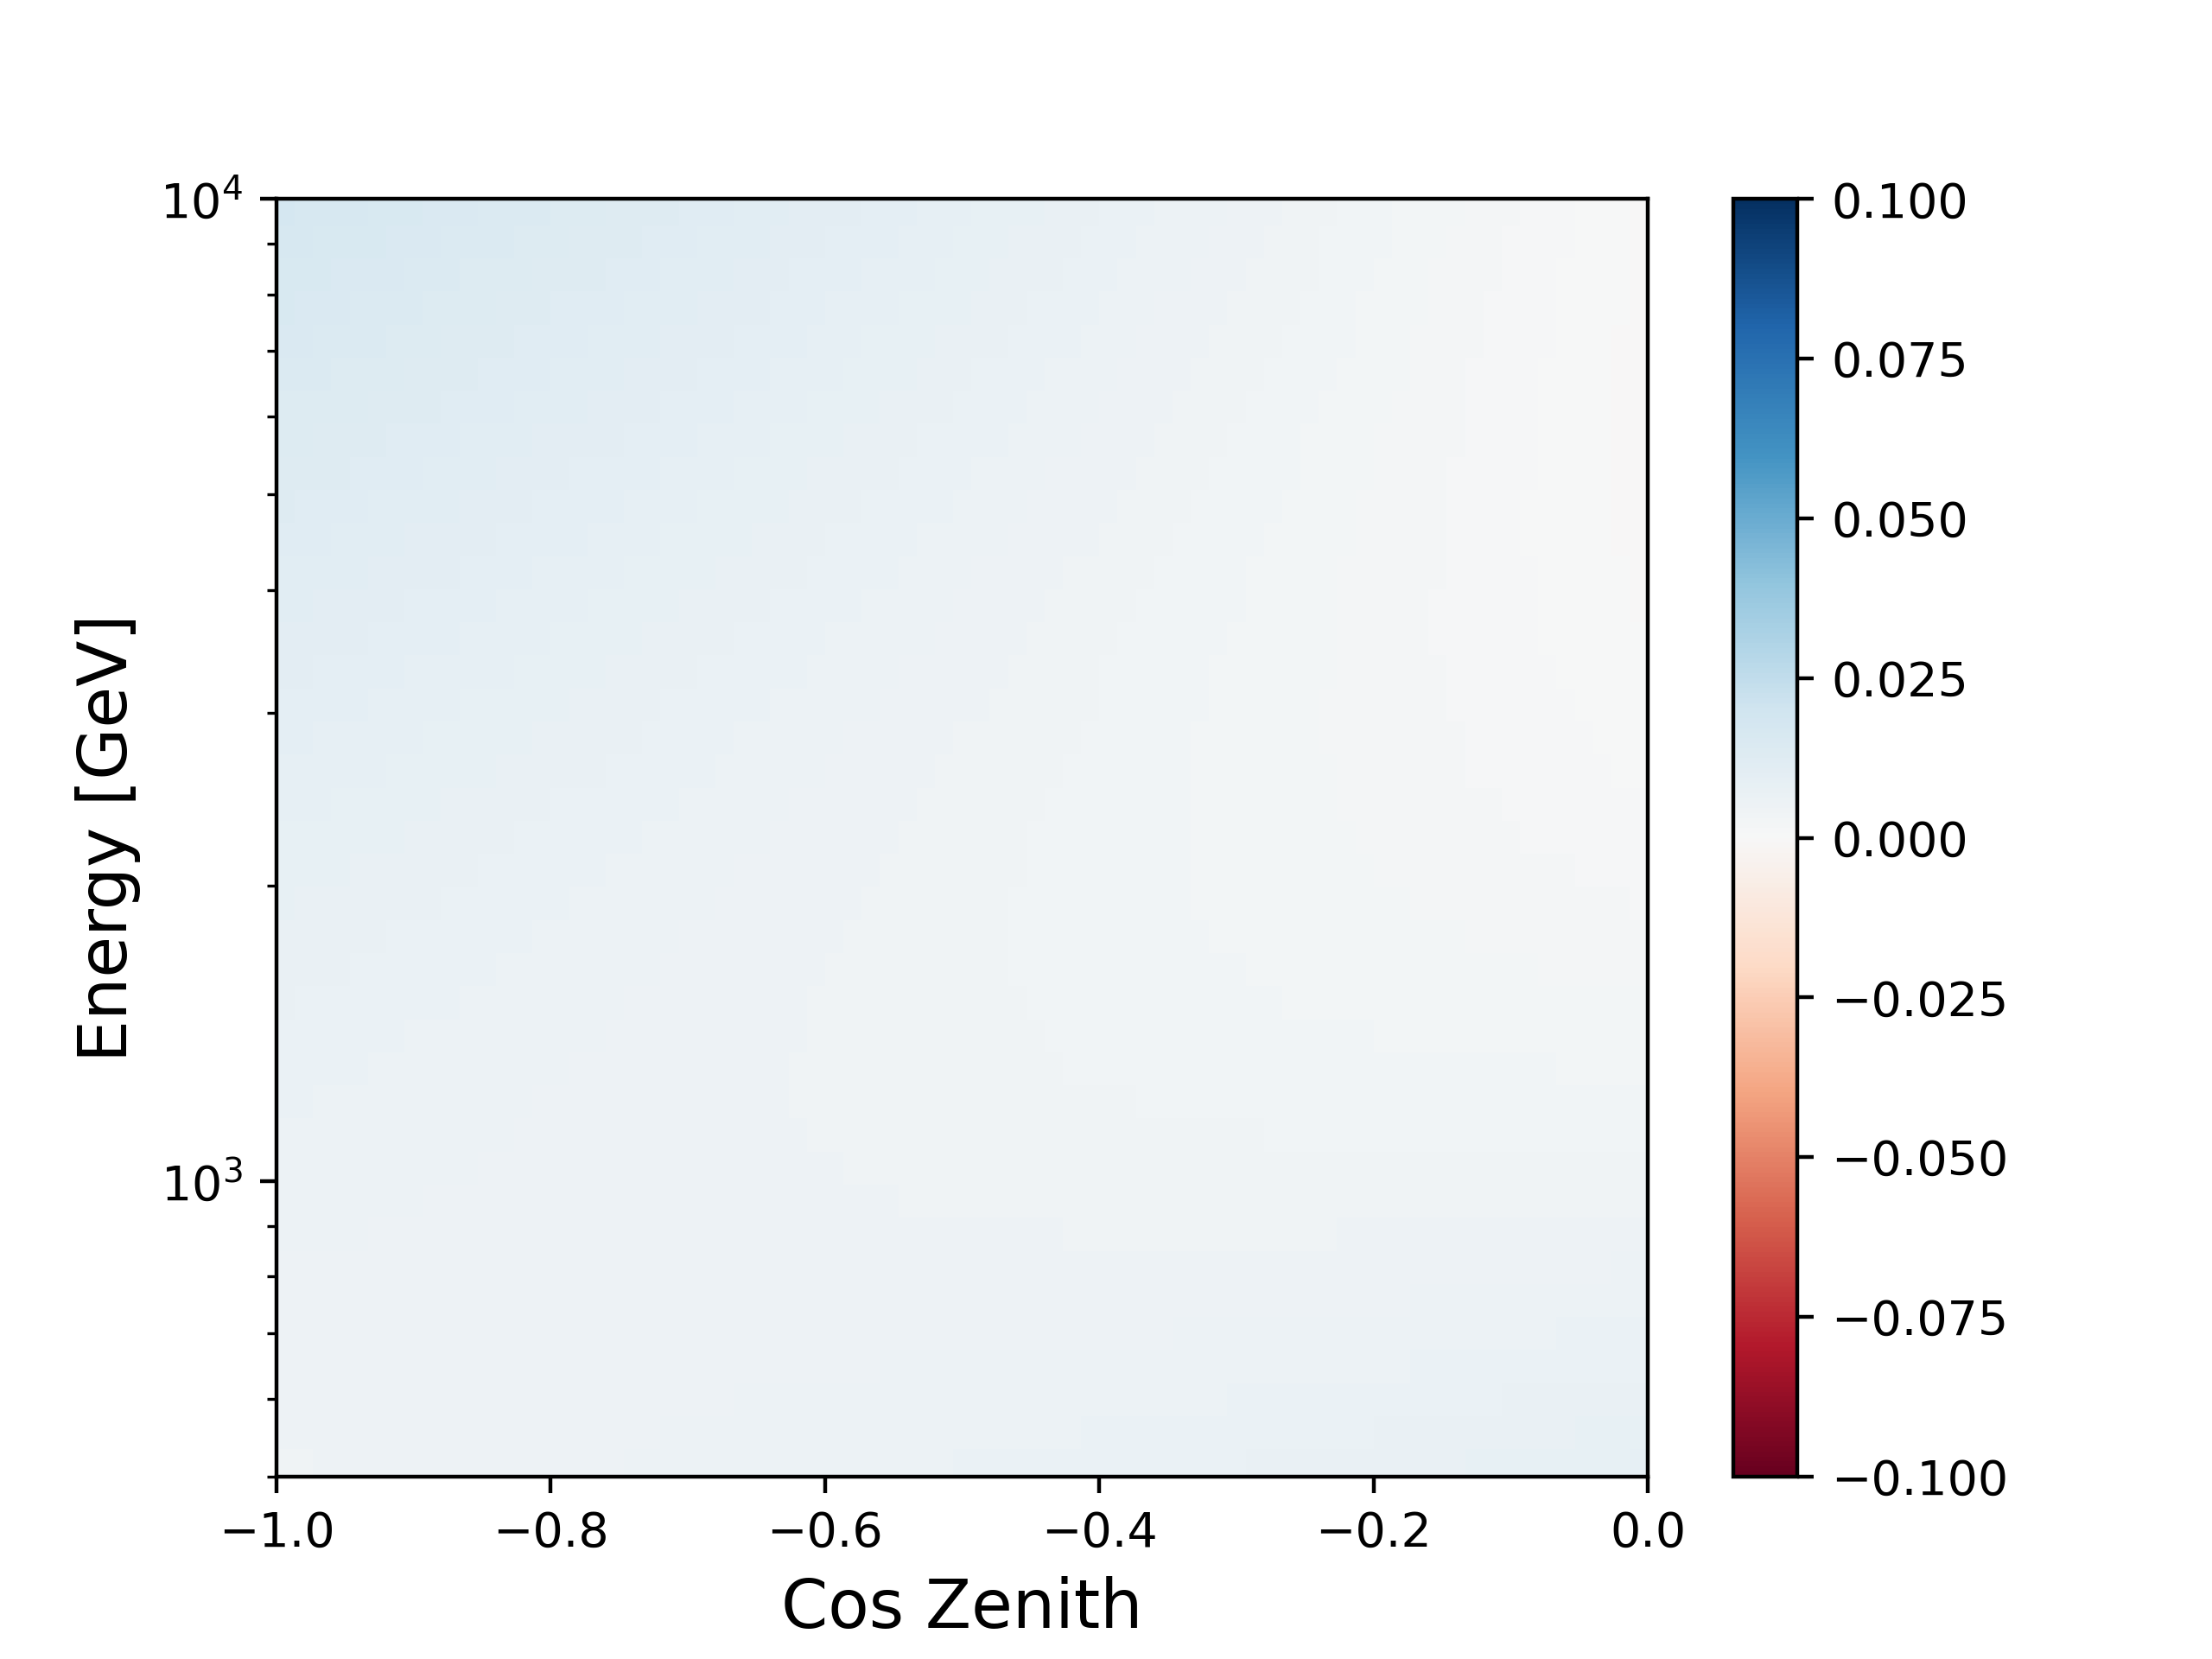
\includegraphics[width=0.3\linewidth]{figures/spline_amp02_gradient.png}\\
    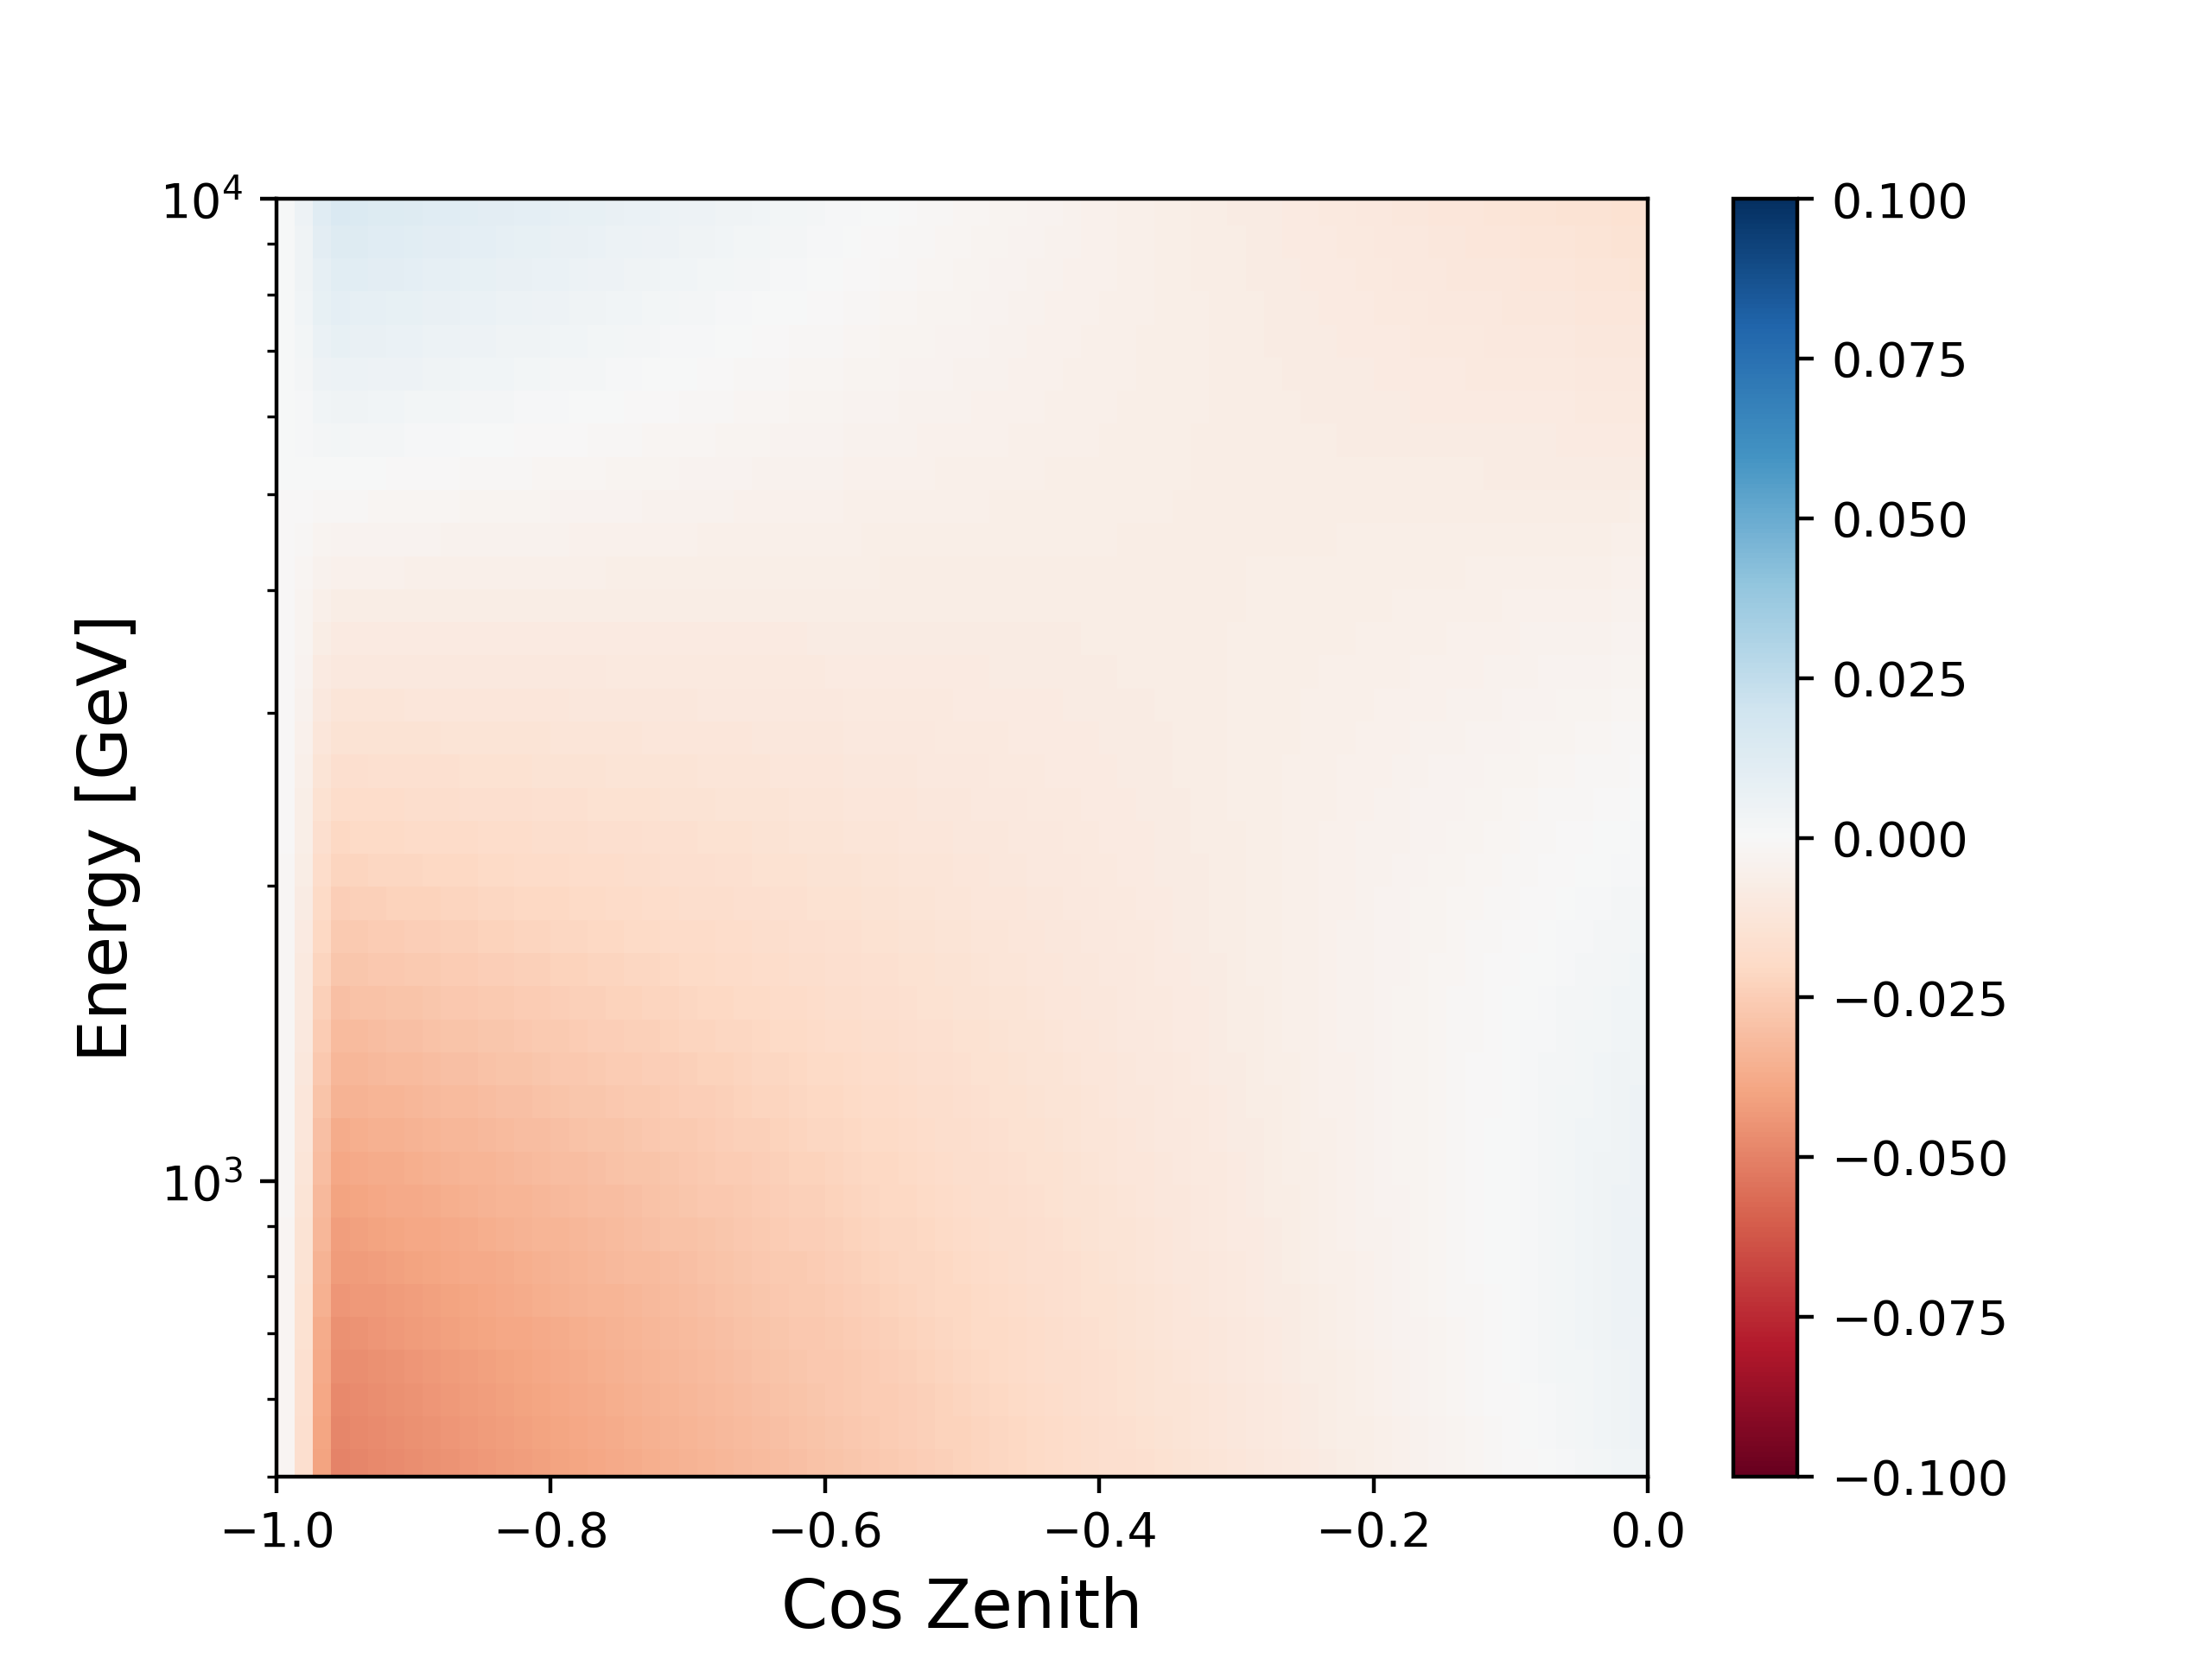
\includegraphics[width=0.3\linewidth]{figures/spline_amp03_gradient.png}%
    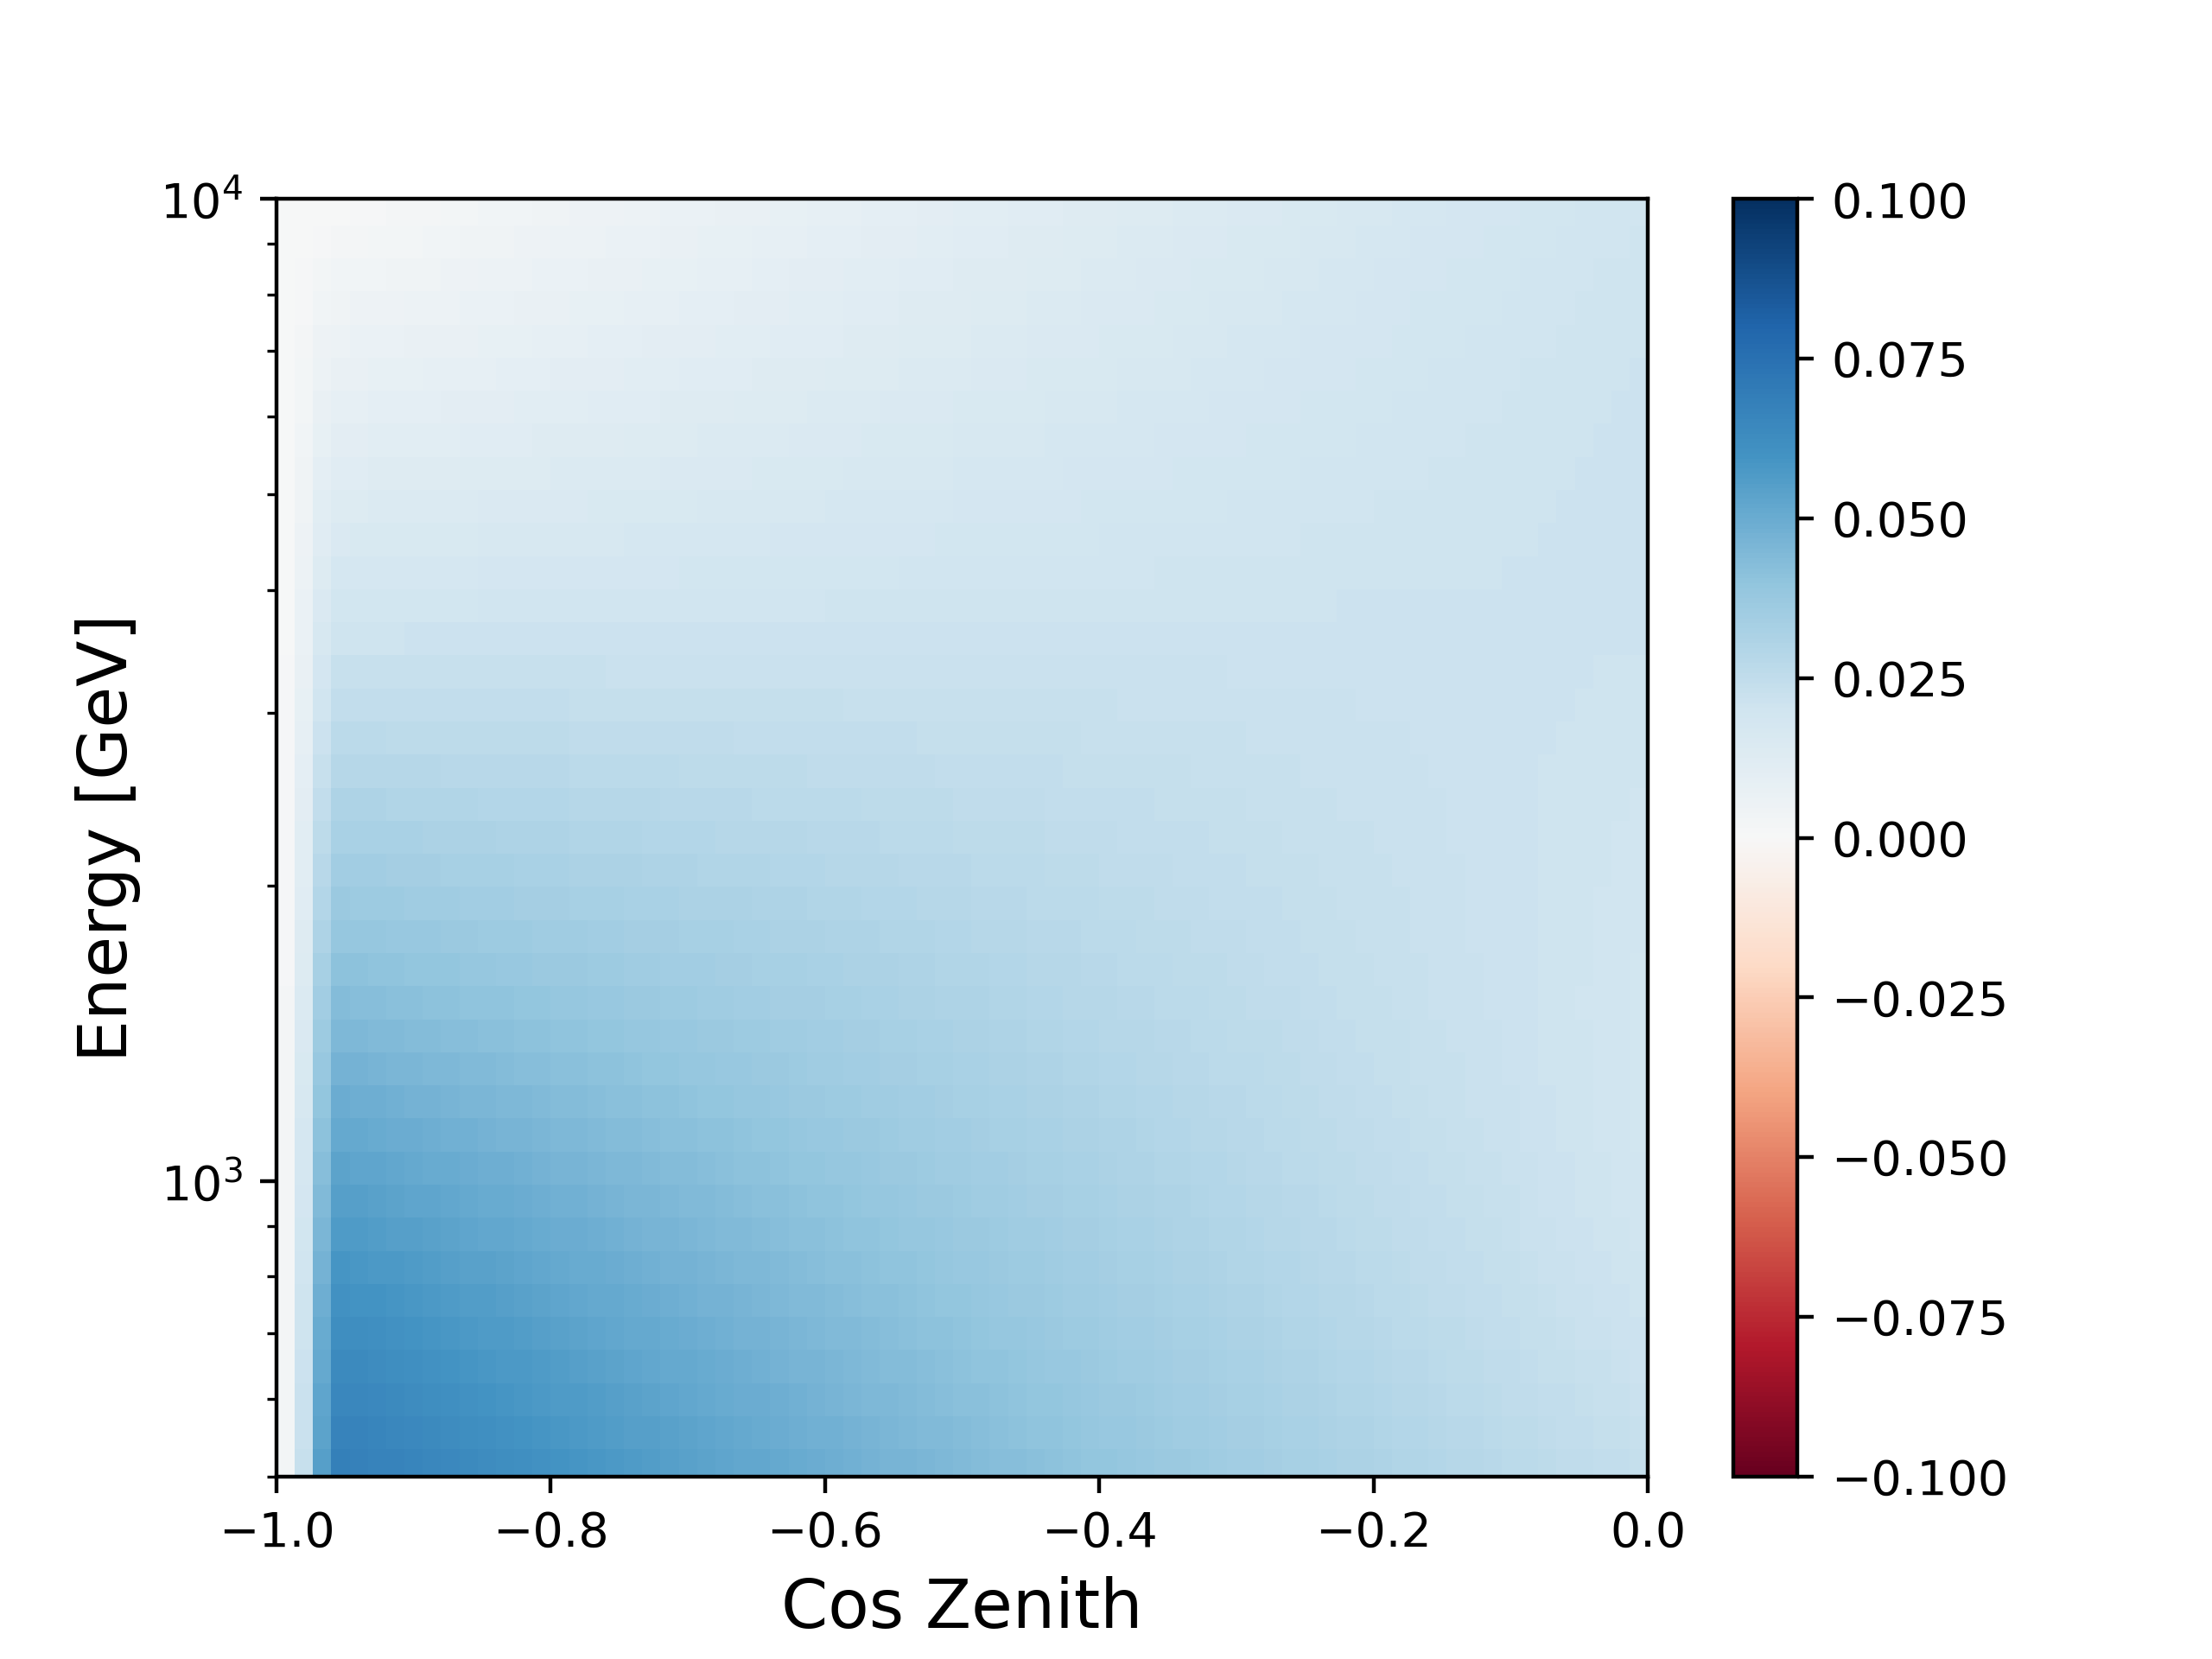
\includegraphics[width=0.3\linewidth]{figures/spline_amp04_gradient.png}%
    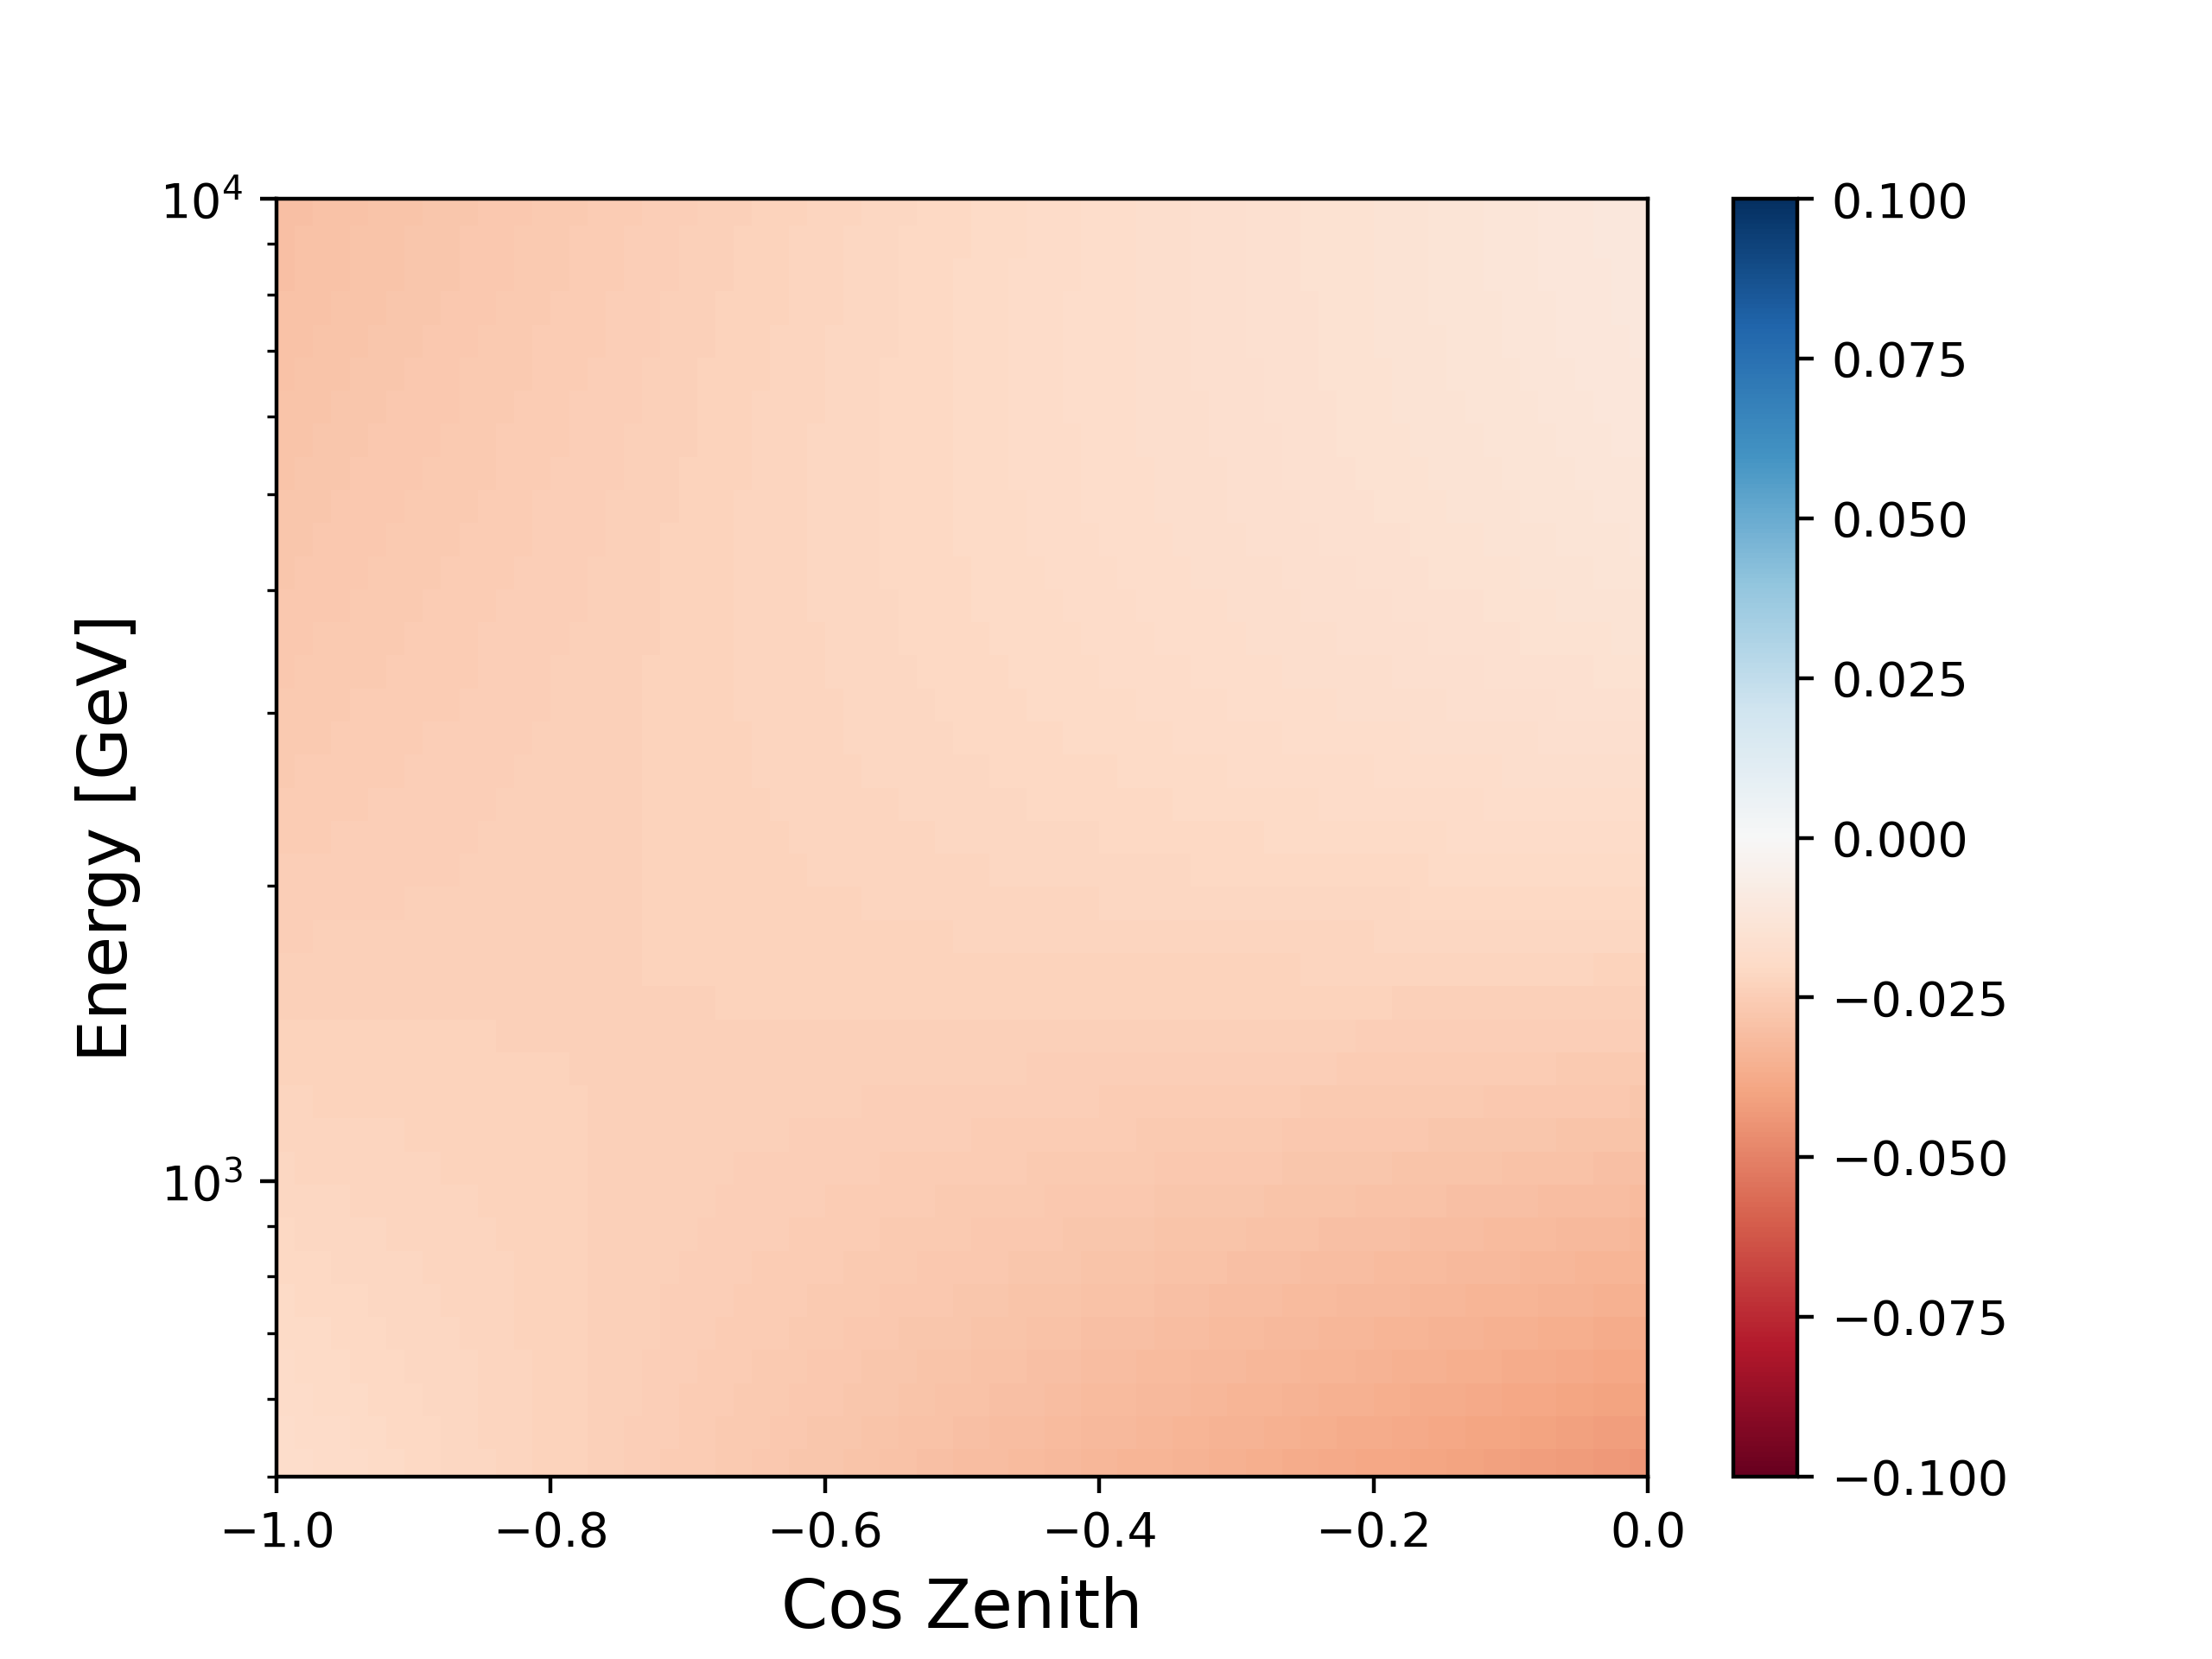
\includegraphics[width=0.3\linewidth]{figures/spline_phase01_gradient.png}\\
    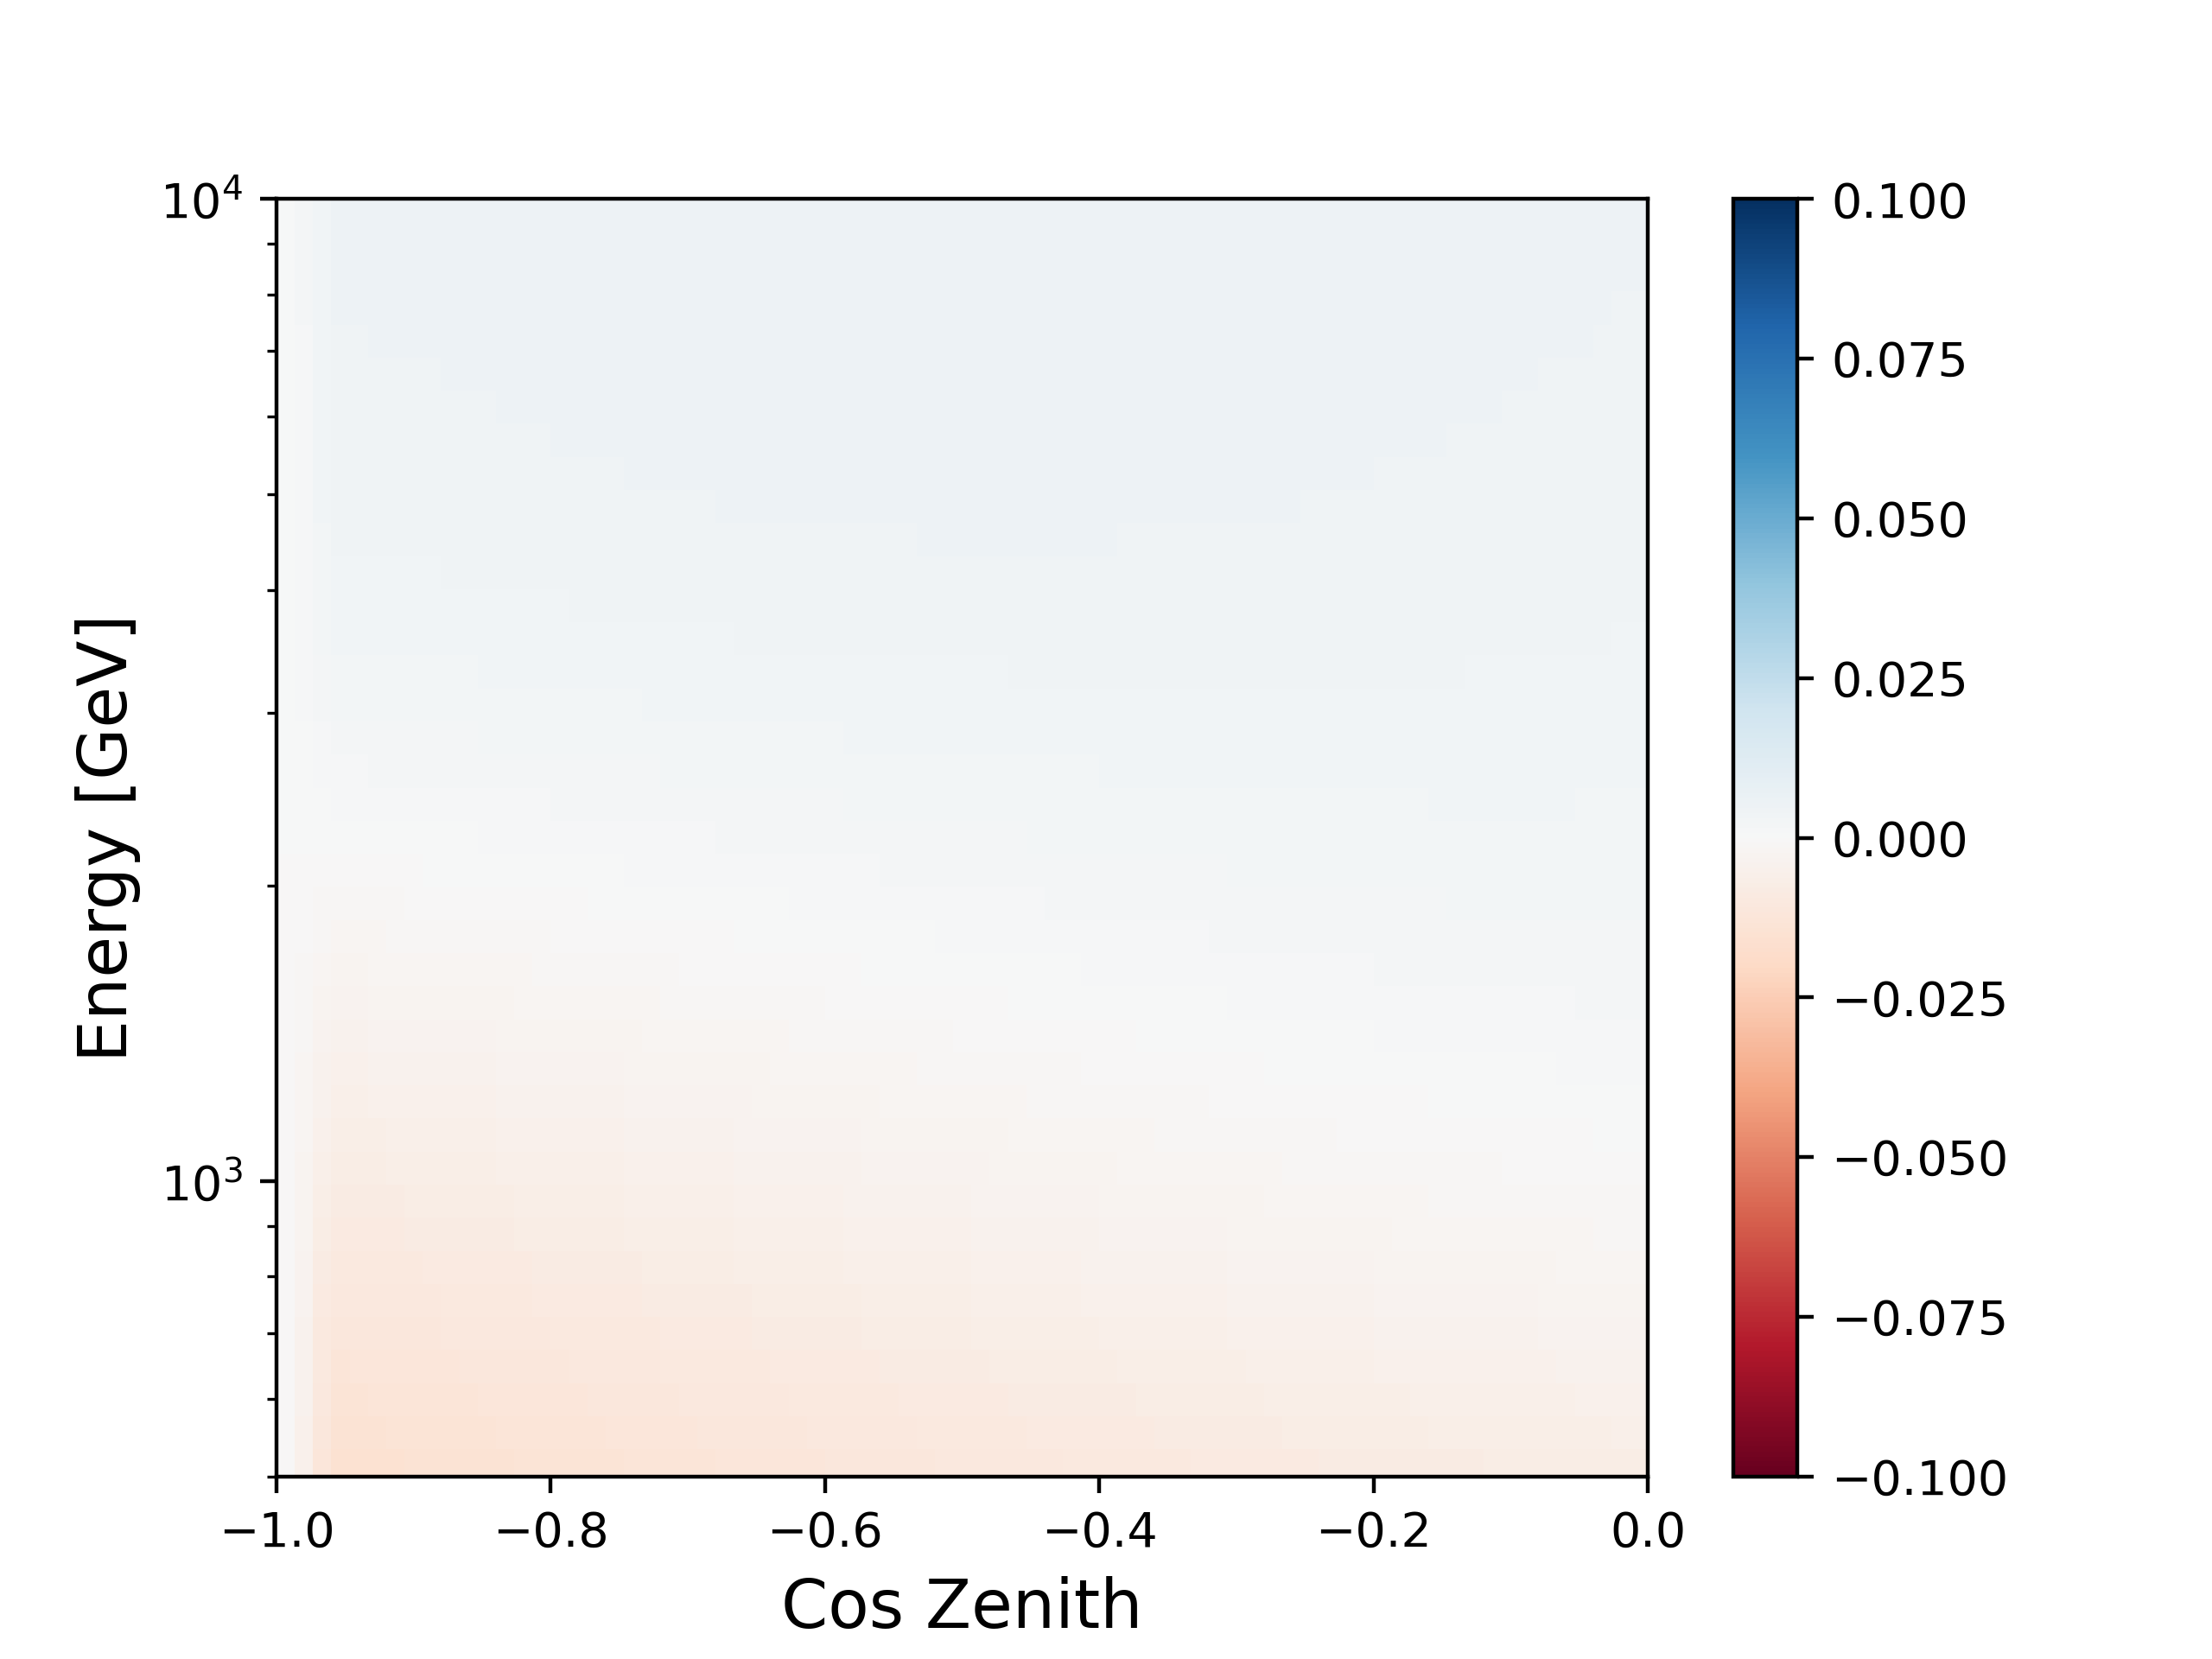
\includegraphics[width=0.3\linewidth]{figures/spline_phase02_gradient.png}%
    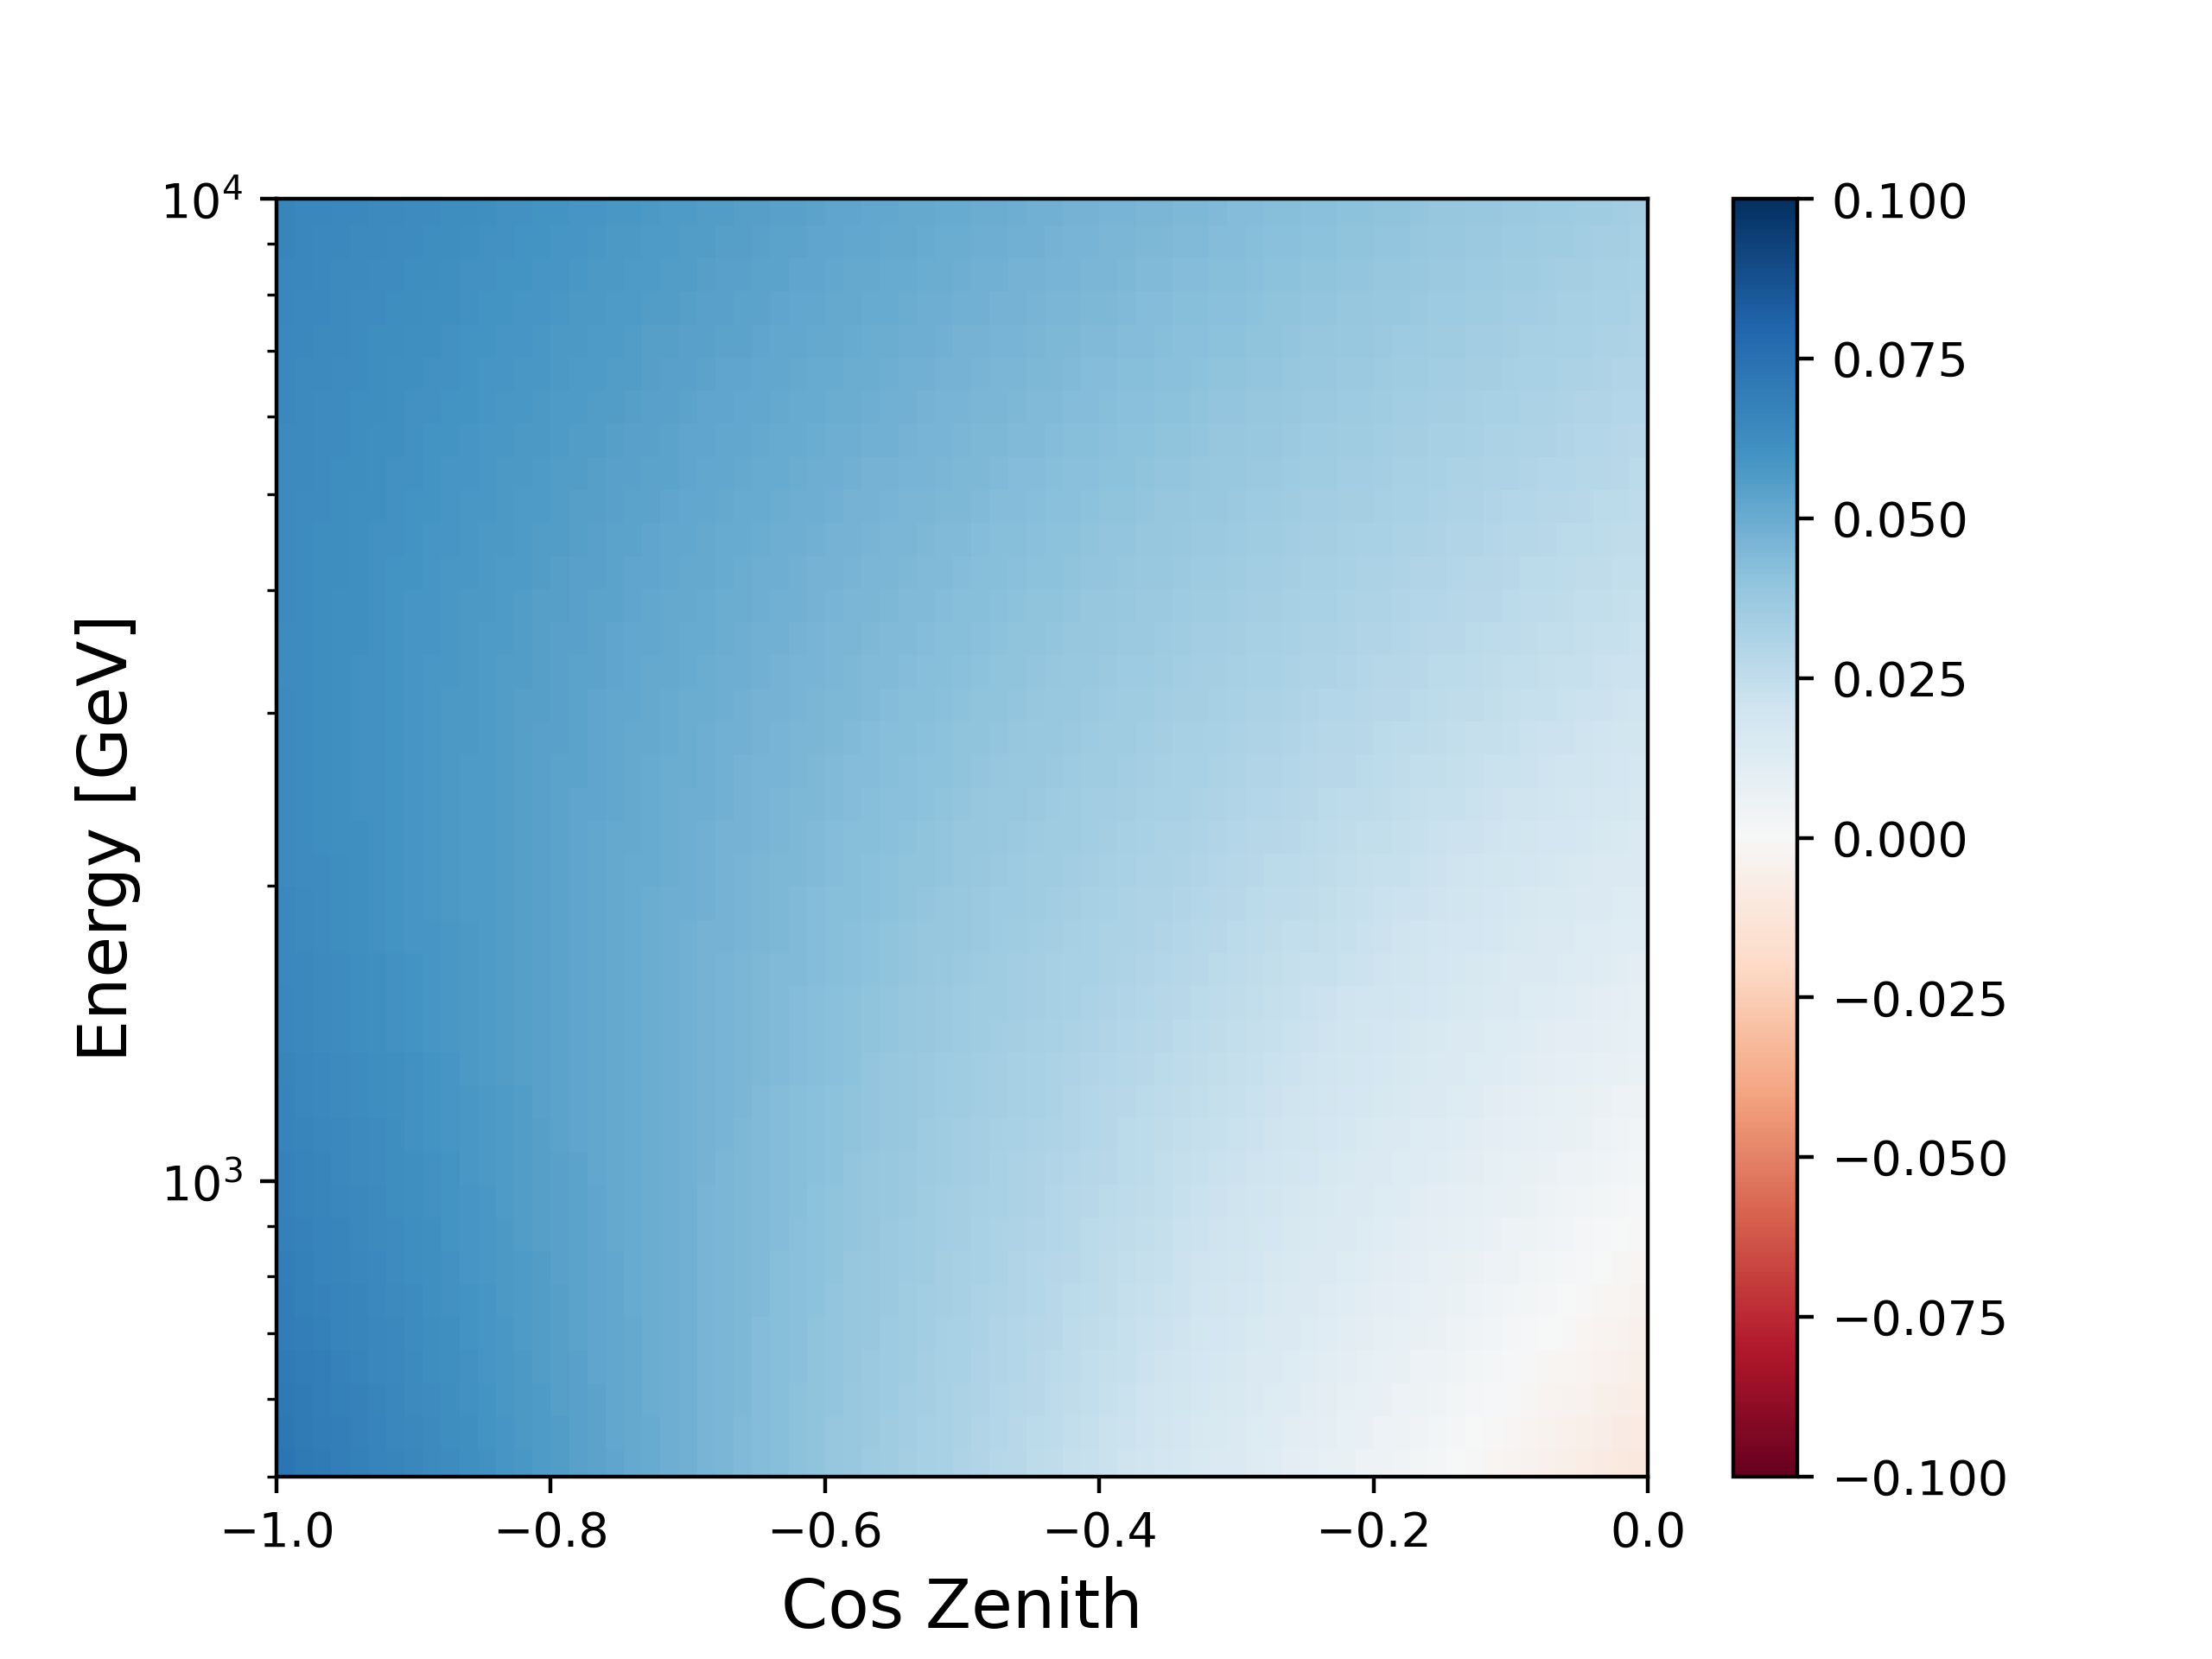
\includegraphics[width=0.3\linewidth]{figures/spline_phase03_gradient.png}%
    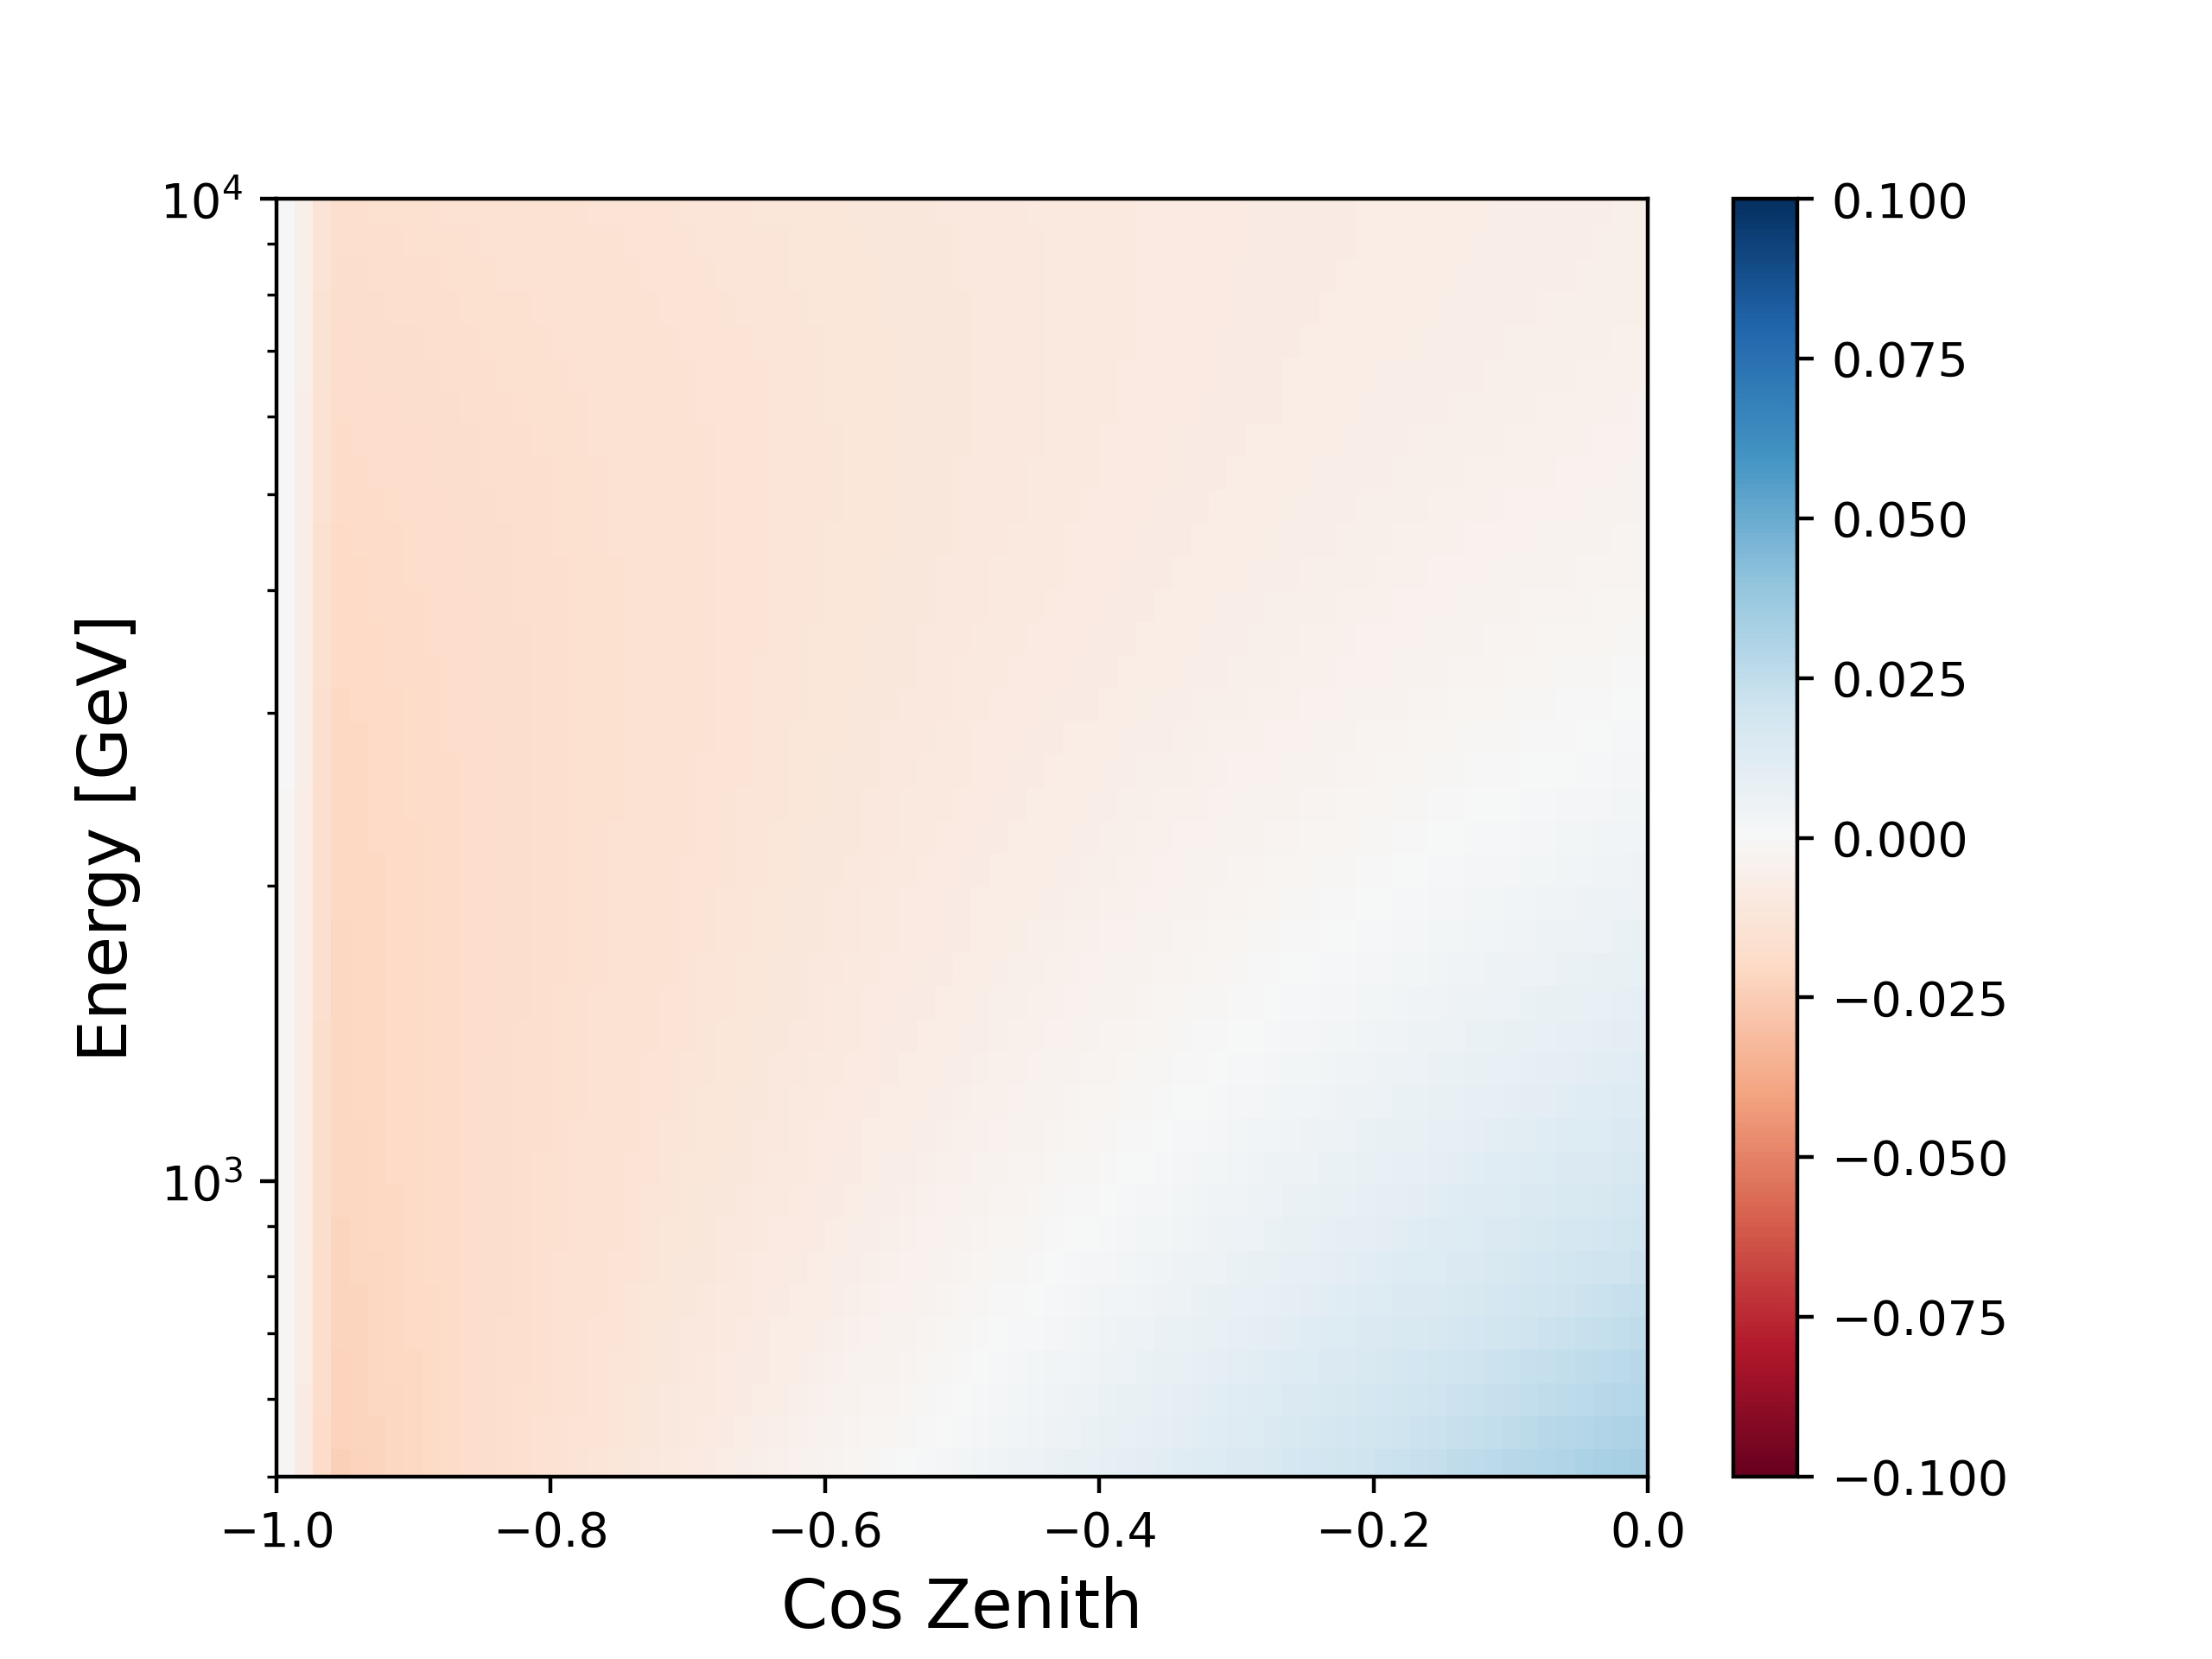
\includegraphics[width=0.3\linewidth]{figures/spline_phase04_gradient.png}
    \caption{Evaluations of the Photospline spline-fits to the 2D gradients as functions of energy and zenith. Left to right from top to bottom: Amplitude 0, Amplitude 1, Amplitude, 2, Amplitude 3, Amplitude 4, Phase 1, Phase 2, Phase 3, Phase 4.}\label{fig:gradients}
\end{figure}


\subsection{Hole Ice}

The hole ice represents a bubbly, refrozen region of ice around the DOMs. 
The bubbles, which formed during the refreezing, greatly decrease the scattering length of light. 
This has the effect of changing the light-acceptance of the DOMs as a function of photon incident angle. 
A plethora of different angular acceptance curves existed from various different calibration studies done to understand this region of the ice; and work was carried out to approximate these different curves and the space they spanned. 
Spline-fits were carried out using seven support points and by forcing the acceptance to zero at the DOM backside (opposite the PMT). 
This resulted in six free, correlated, parameters needed to describe the acceptance curve. 
A principal component analysis was carried out, and it was found that all acceptance curves span a phase space of lower dimensionality. 
Only two components were needed to describe the space of angular acceptance curves, and those were named $p_{0}$ and $p_{1}$.
In doing so, a small amount of error is introduced, though the overall uncertainty on the hole ice that remains is far greater than the introduced error. 

By construction, these parameters' priors are independent.
The effects of varrying these two parameters is then demonstrated in Figures~\ref{fig:holeiceparmas}.

\begin{figure}
    \centering
    \begin{subfigure}{.45\textwidth}
        \centering
        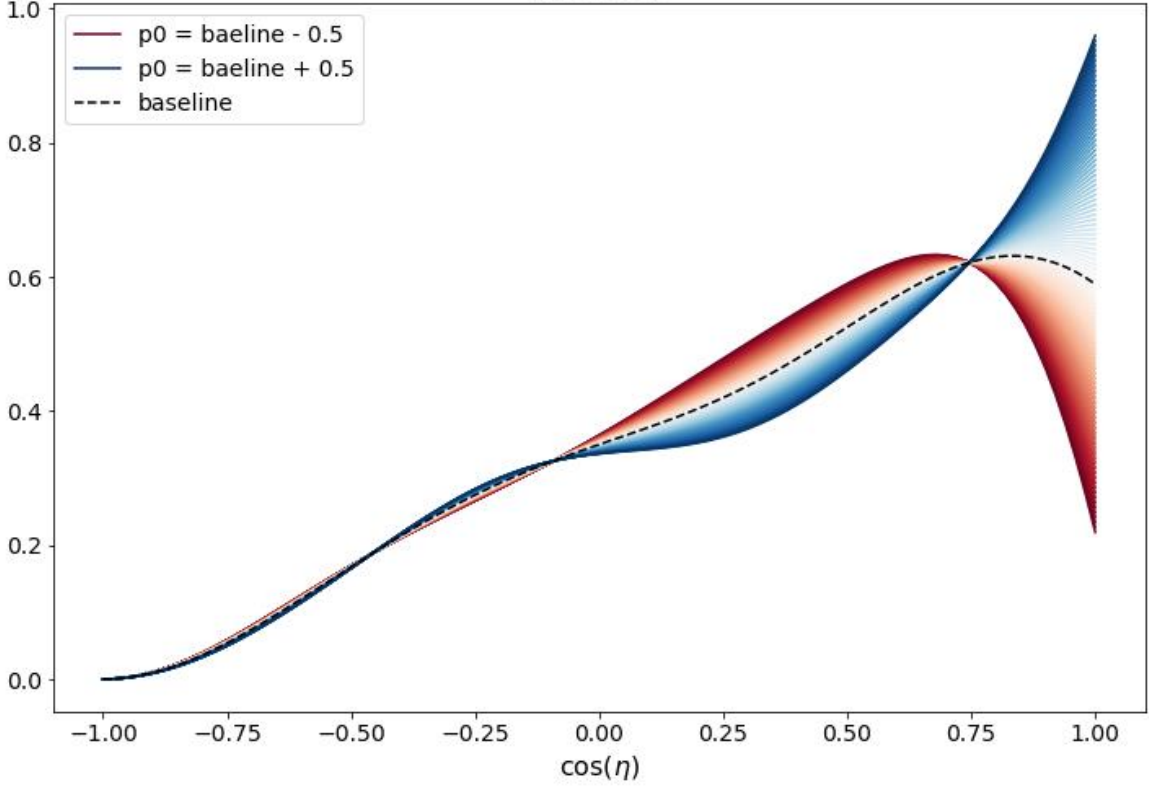
\includegraphics[width=0.95\linewidth]{./figures/holeice_p0.png}
        \caption{A sweep of the unified hole ice model $p_0$ parameter.}
    \end{subfigure}%
    \begin{subfigure}{.45\textwidth}
        \centering
        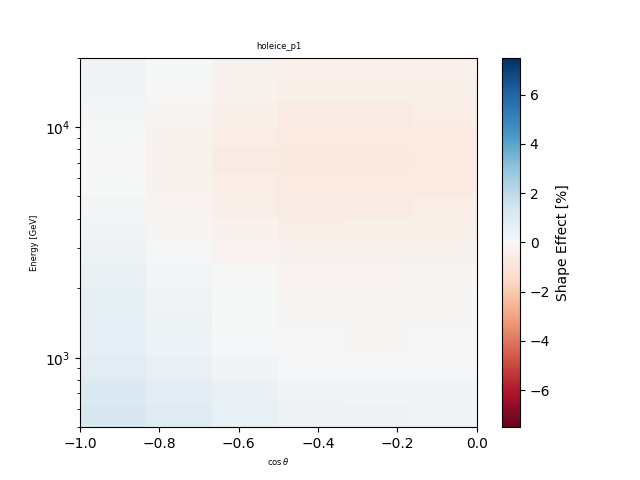
\includegraphics[width=0.95\linewidth]{./figures/holeice_p1.png}
        \caption{A sweep of the unified hole ice model $p_1$ parameter.}
    \end{subfigure}
    \caption{Effects of varrying unified hole ice model parameters. $\eta$ represents angle of photon incidence on the DOM; -1 is the DOM backside, and +1 is the DOM PMT face.}\label{fig:holeiceparmas}
\end{figure}

For each batch of ten simulated MC events these parameters $p_{0}$ and $p_{1}$ are randomly sampled from their priors. 
The angular acceptance of the DOMs in CLSim is then manually adjusted according to the new hole ice model, and the photon propagation is then carried out. 
The remainder of the MC simulation chain is then performed.

The final-level MC is then weighted, one at a time, to the conventional, prompt, and astrophysical neutrino fluxes. 
The snowstorm technique is applied to this MC sample, and the 1D gradients in reconstructed space are shown in Figure FIG. 

\subsection{Atmospheric Neutrino Flux}

Daemonflux and such

\subsection{Atmospheric Density}

\subsection{Keon-nuclei Total Cross Section}

\subsection{Astrophysical Neutrino Flux}

\subsection{Neutrino-Nucleon Interaction}

\end{document}